\cleardoublepage
\appendix
\chapter{Data Report}

\section{Continuous Variables - Frequency Plots}
\label{sec:continuous}
Figure~\ref{continuous-1} to~\ref{continuous-18} display the distribution of the different continuous features. 

\begin{figure}[ht]
    \begin{center}
    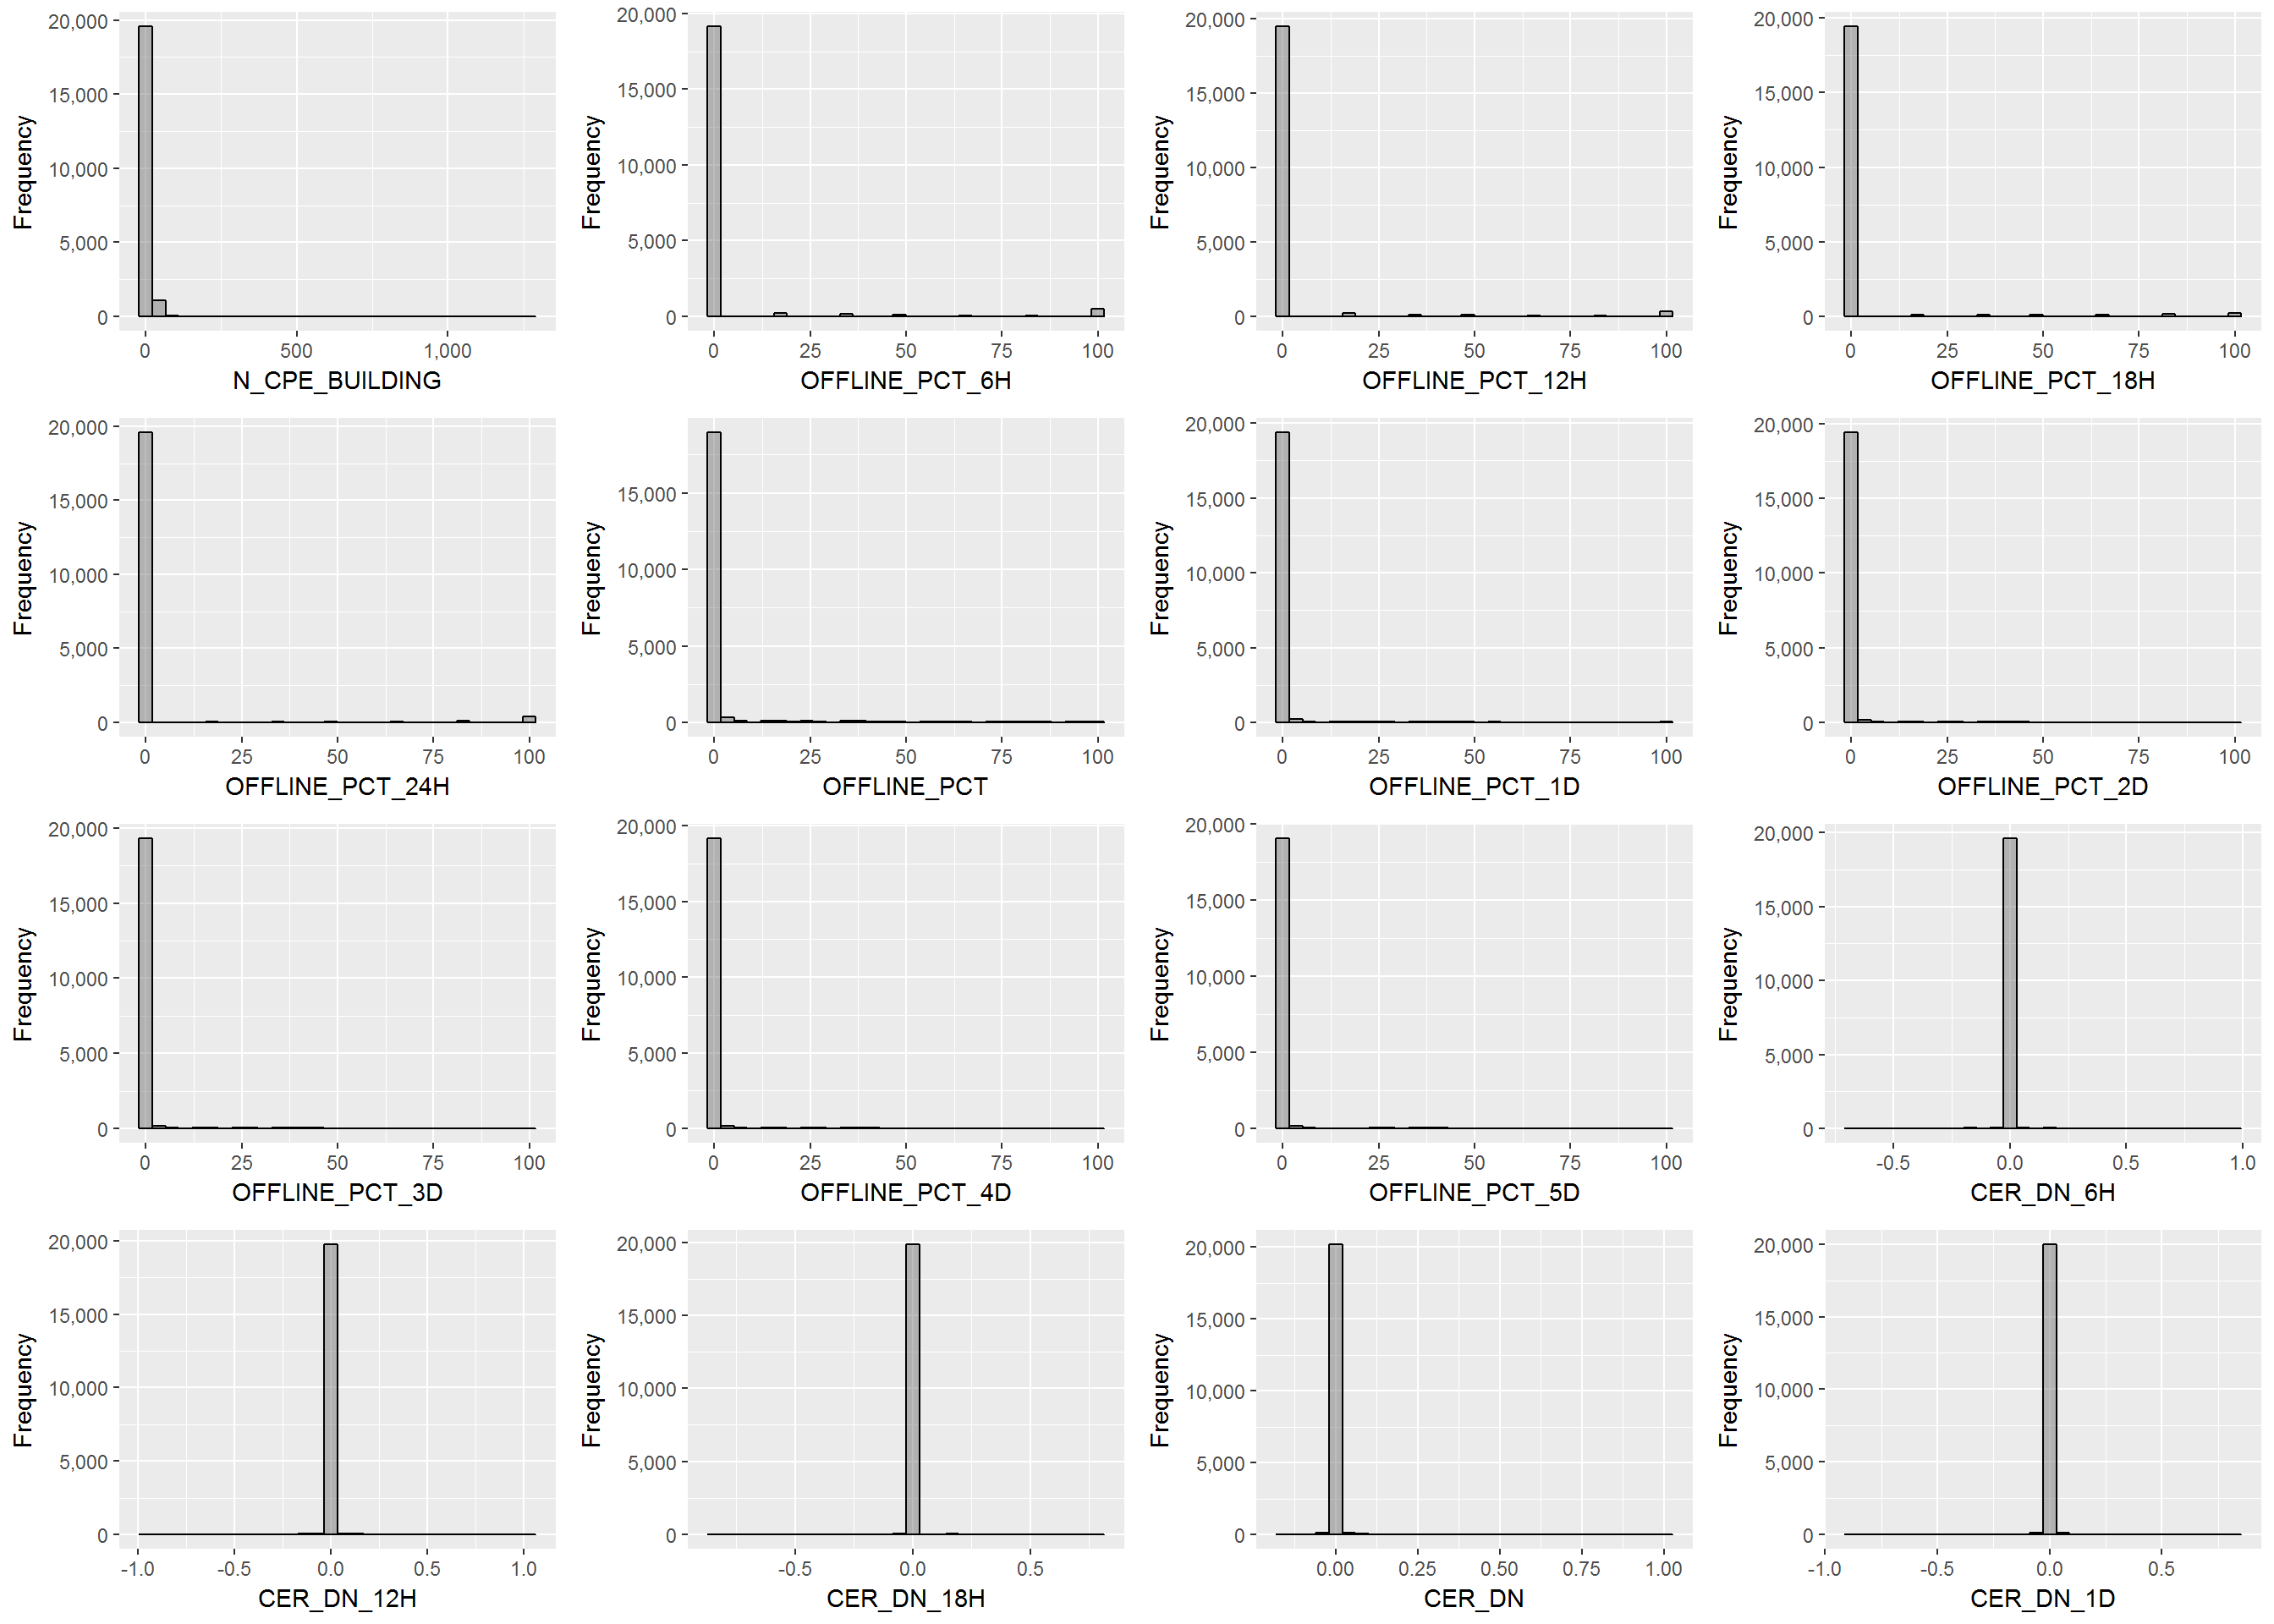
\includegraphics[width=1\linewidth]{continuous-1}
    \end{center}
    \caption{Part 1}
    \label{continuous-1}
\end{figure}

\begin{figure}[ht]
    \begin{center}
    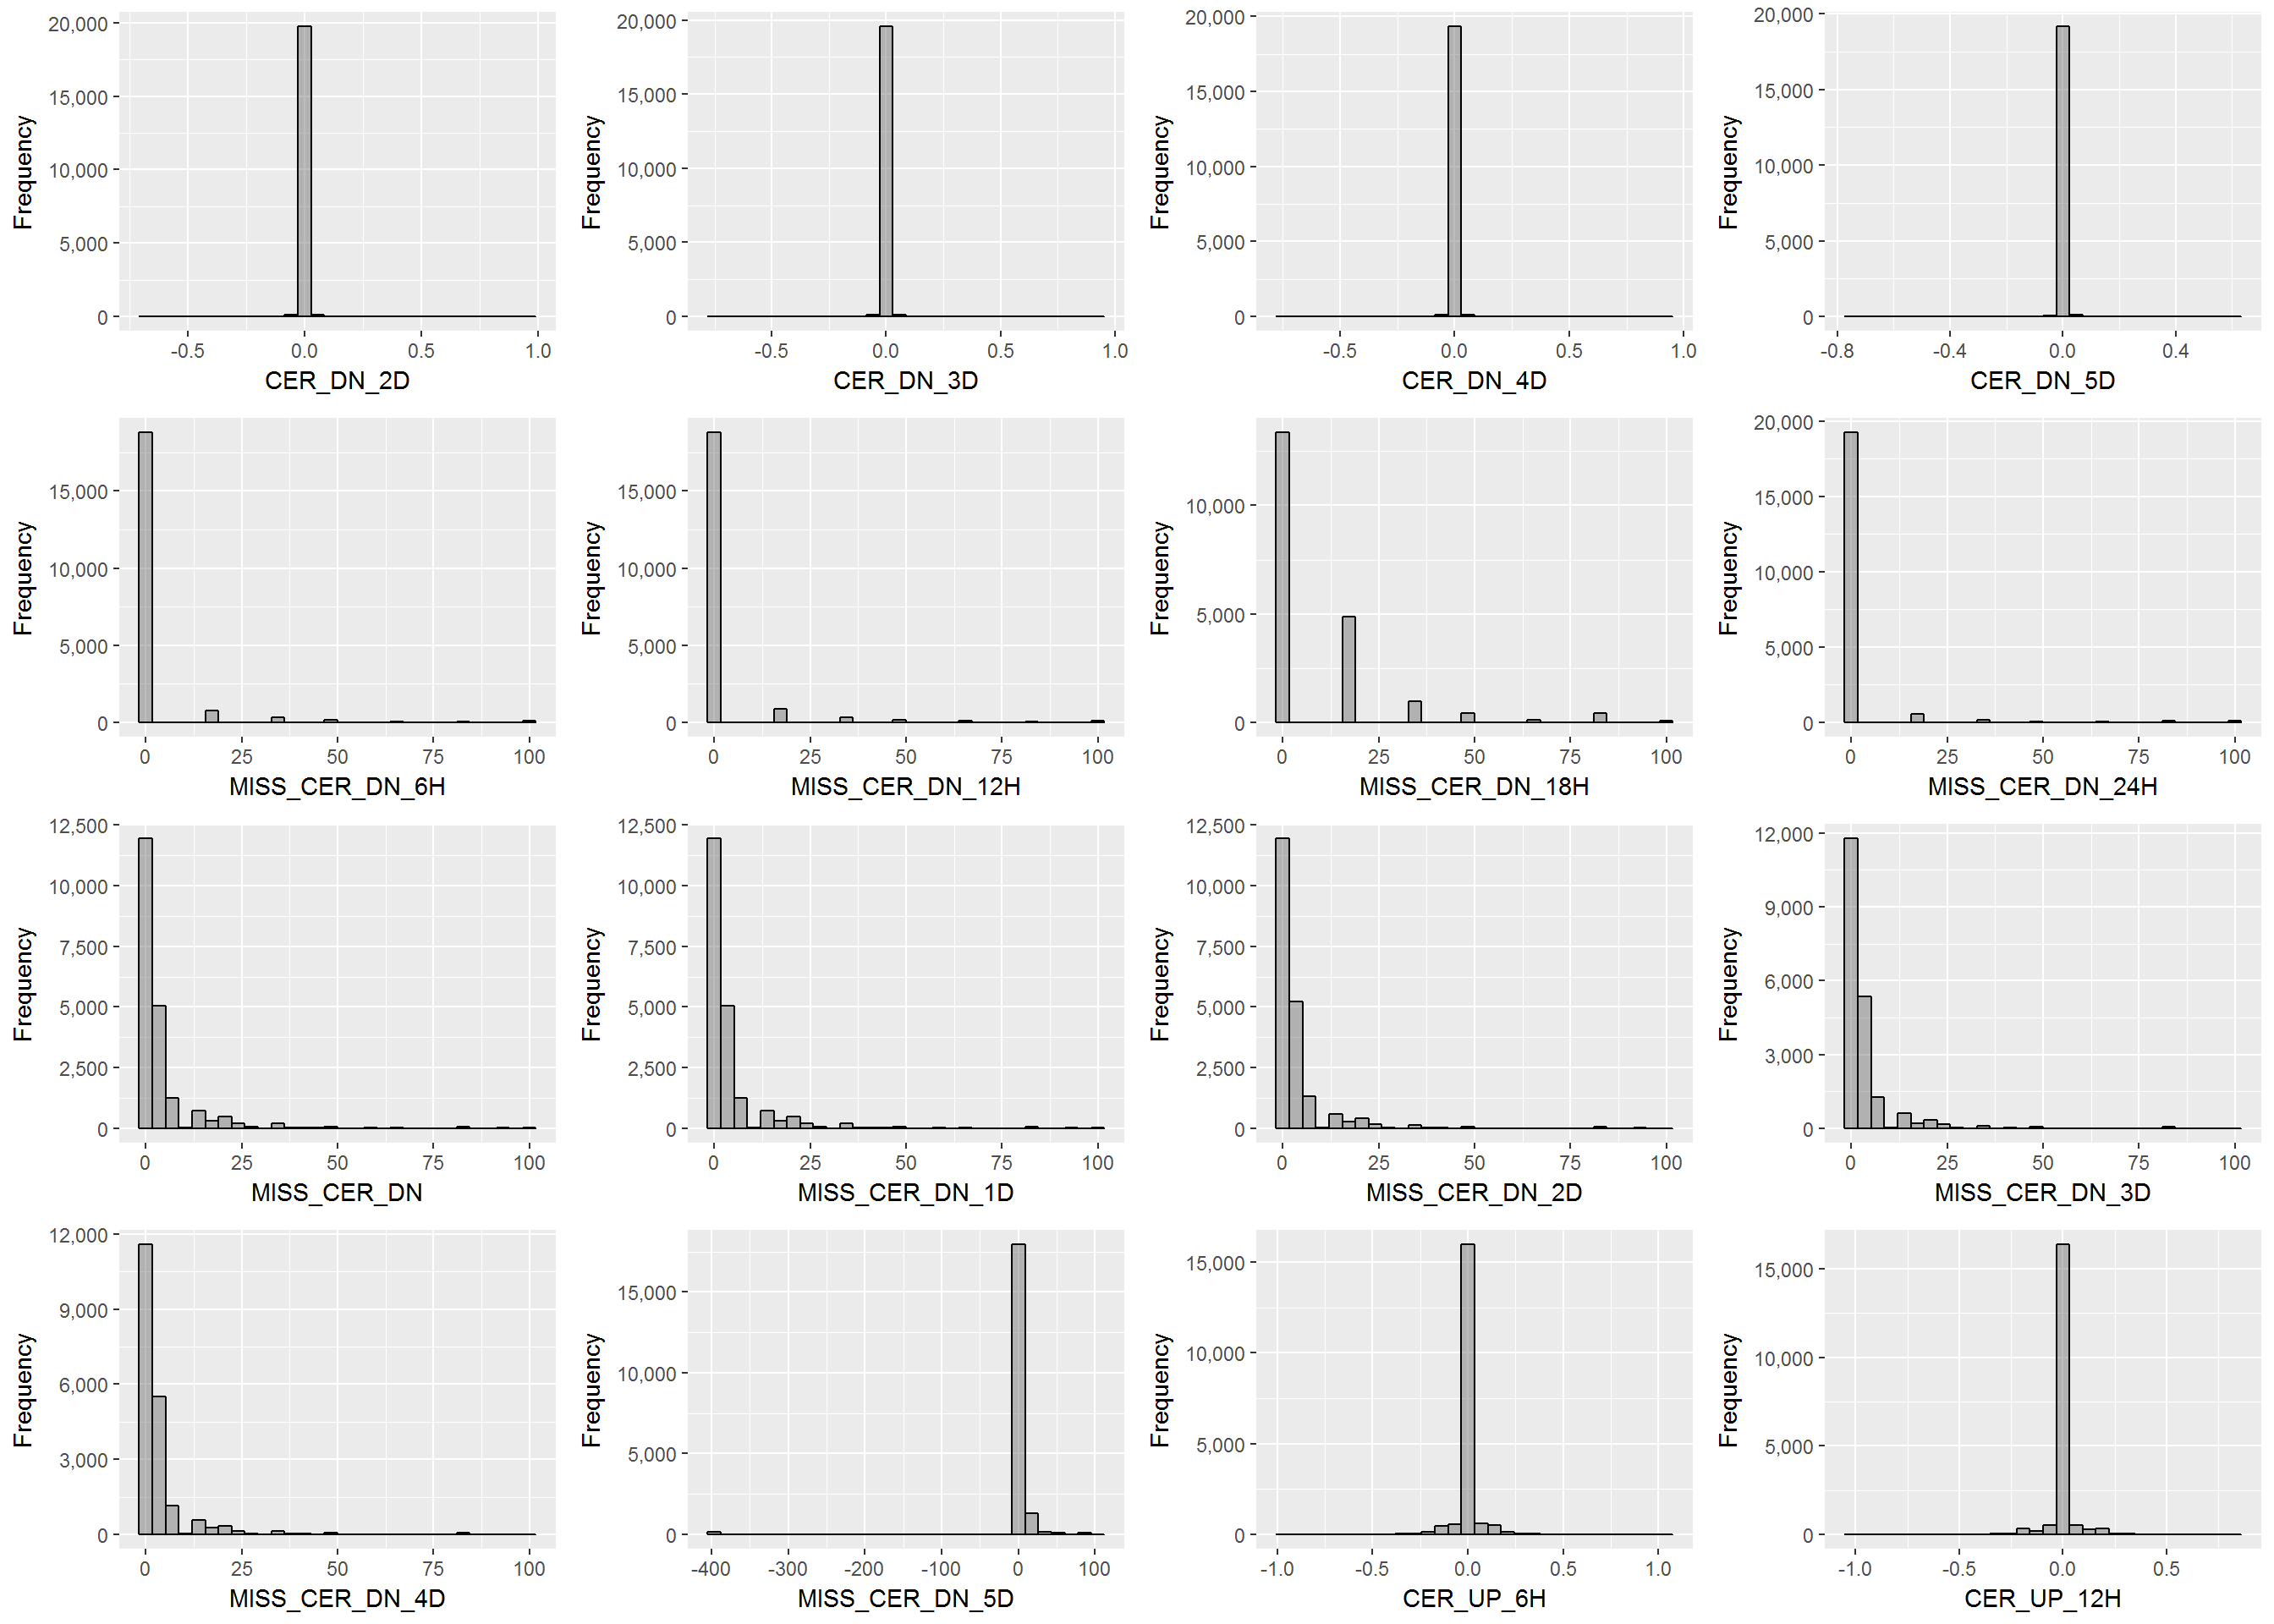
\includegraphics[width=1\linewidth]{continuous-2}
    \end{center}
    \caption{Part 2}
    \label{continuous-2}
\end{figure}

\begin{figure}[ht]
    \begin{center}
    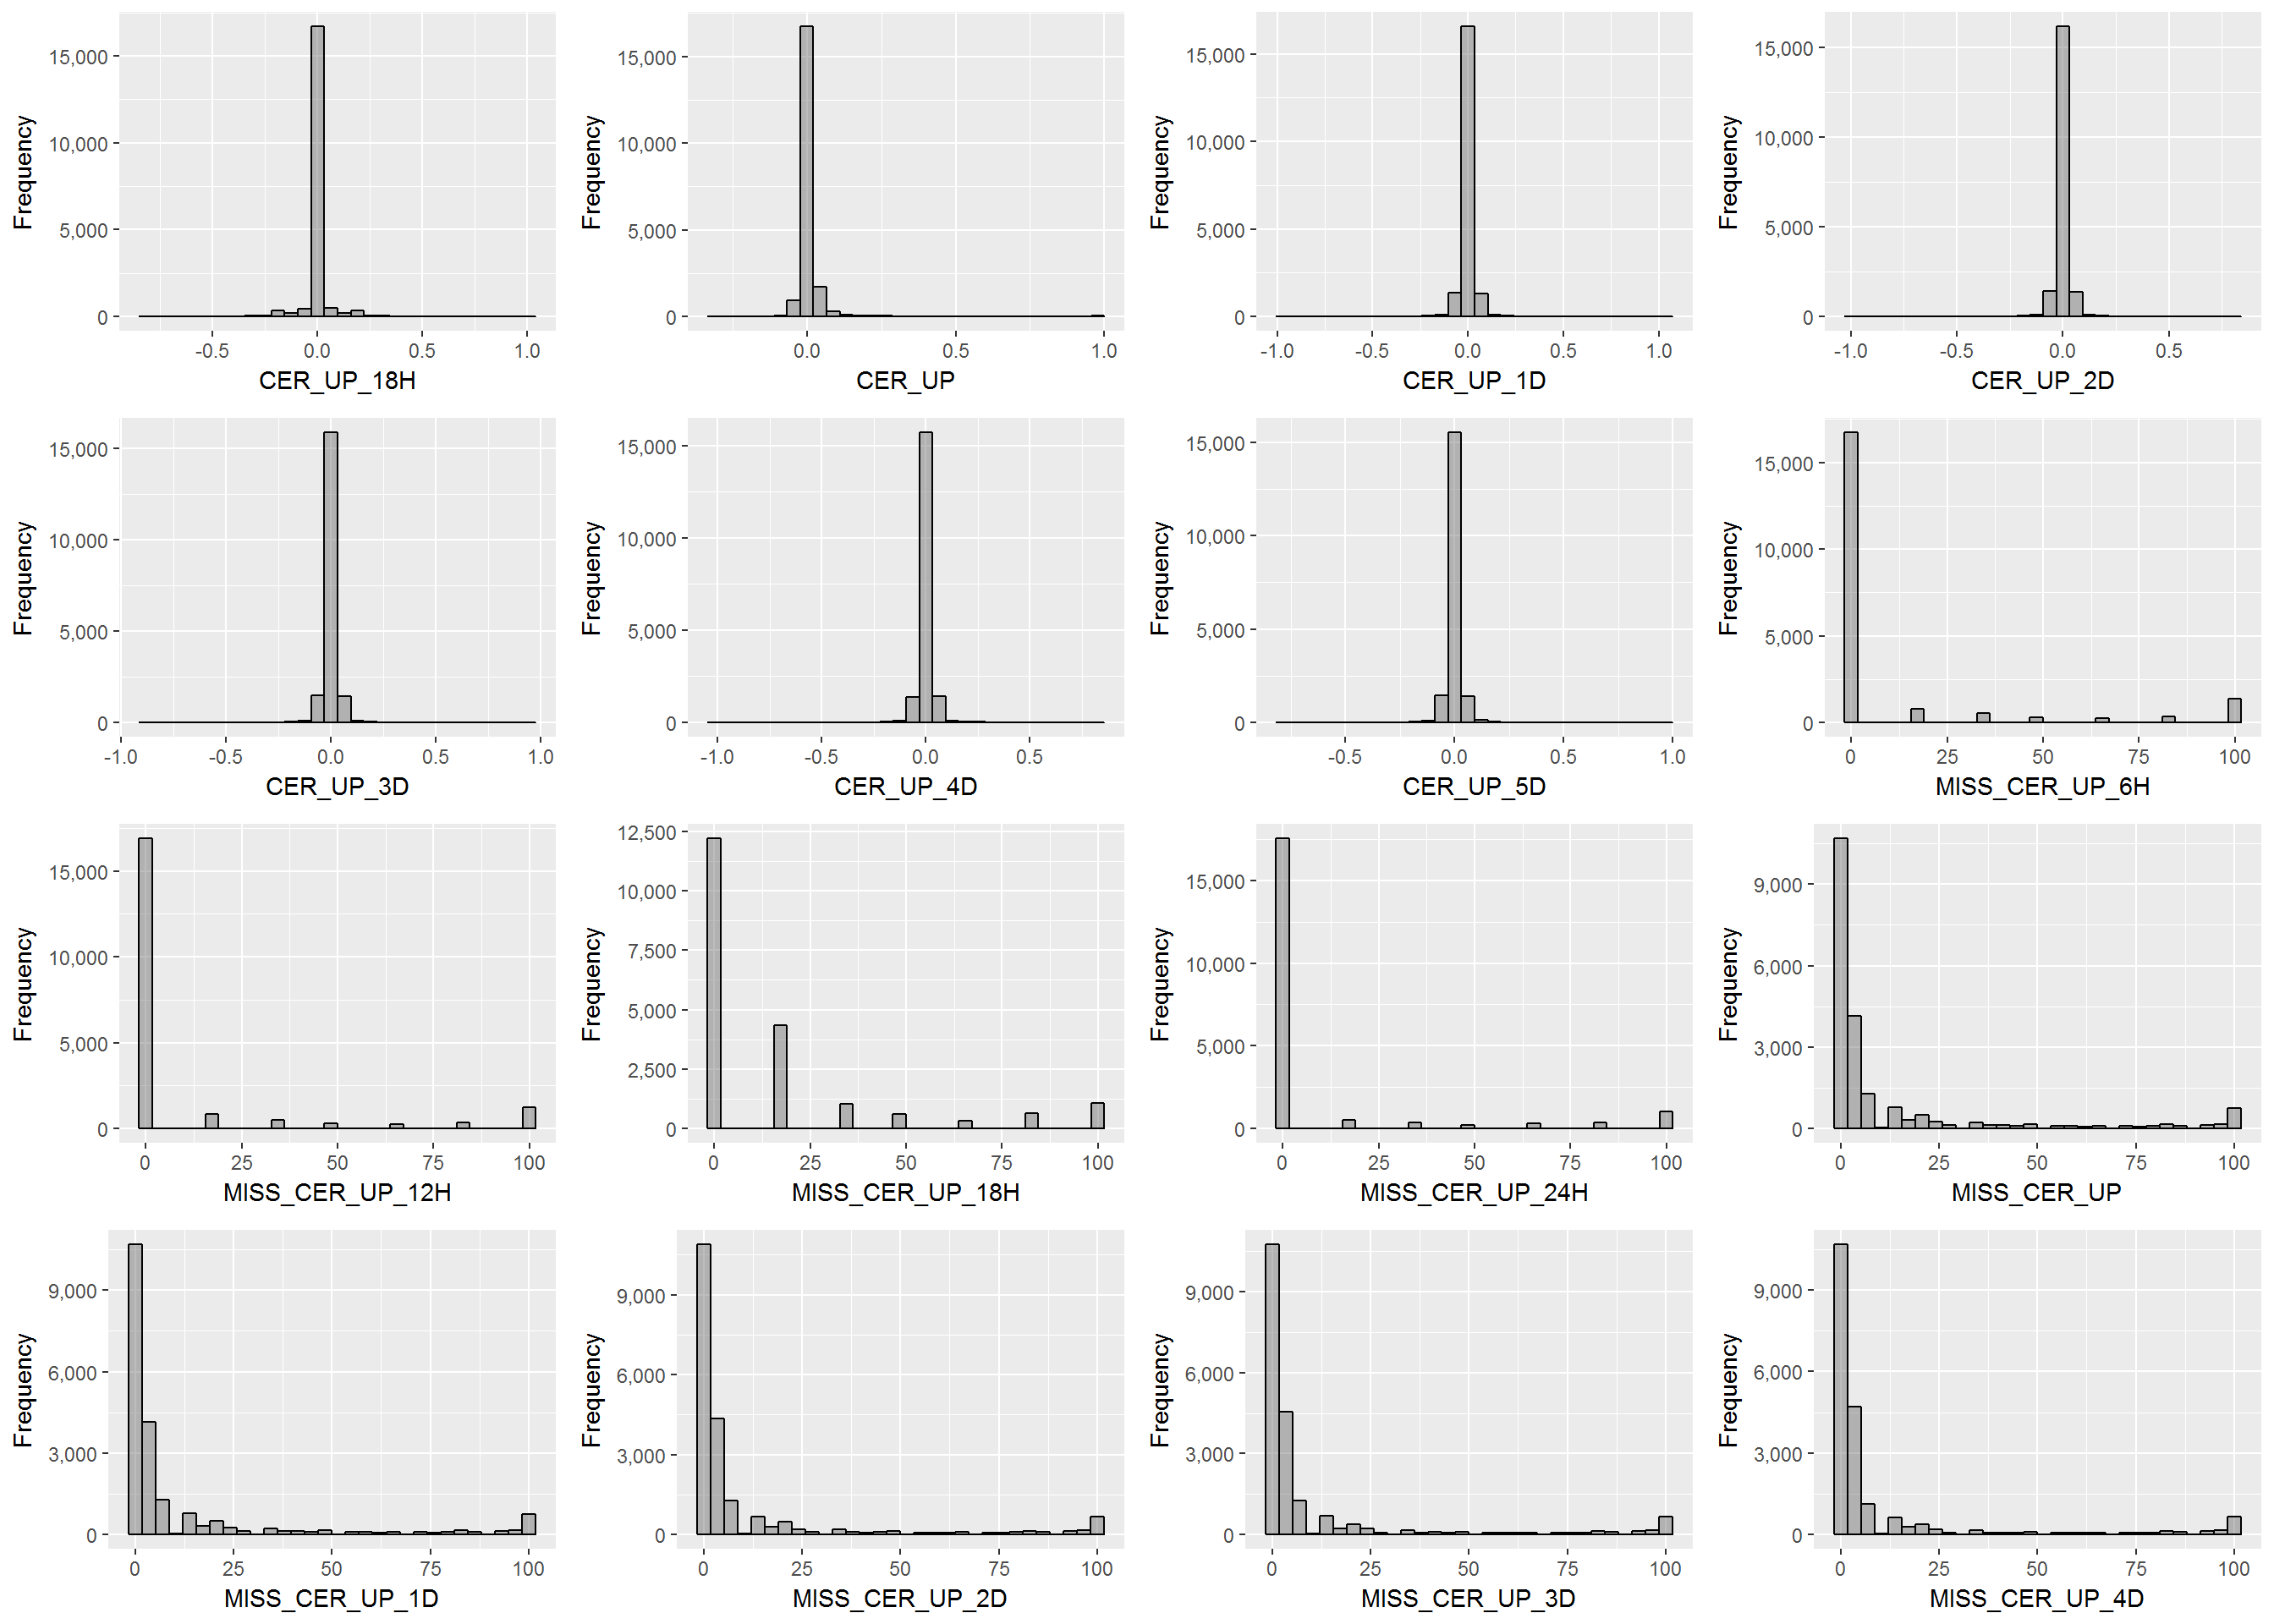
\includegraphics[width=1\linewidth]{continuous-3}
    \end{center}
    \caption{Part 3}
    \label{continuous-3}
\end{figure}

\begin{figure}[ht]
    \begin{center}
    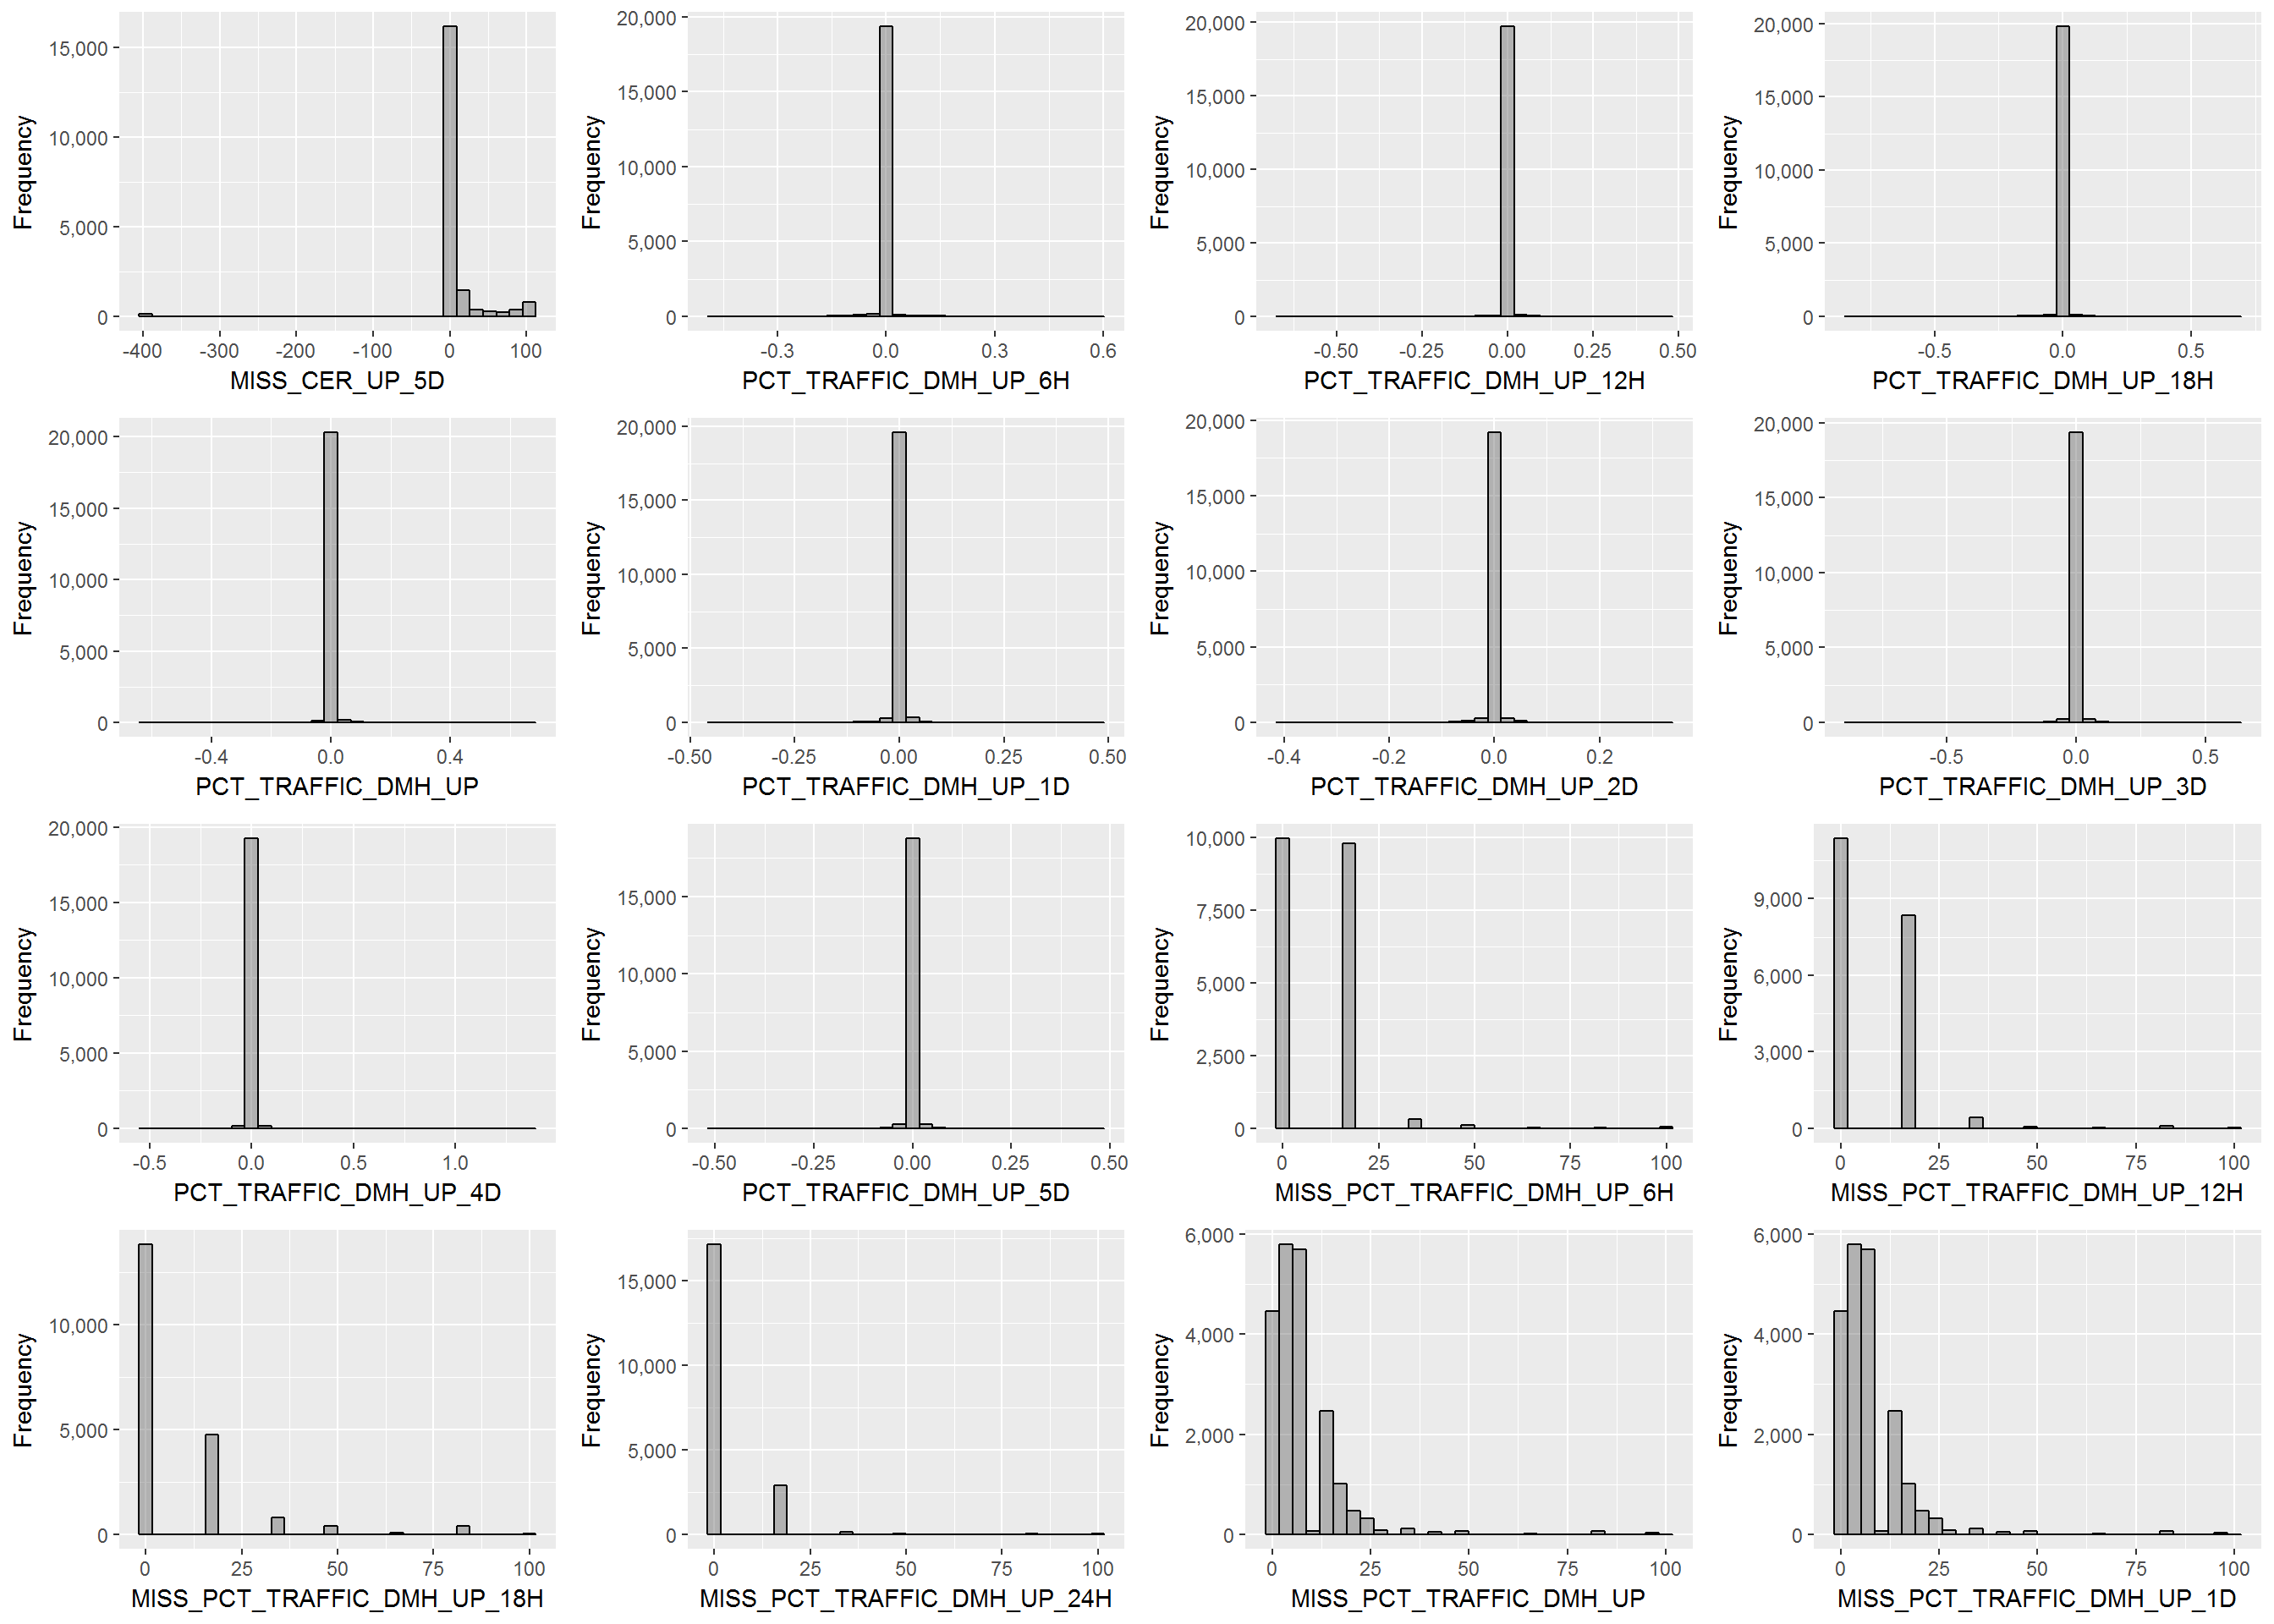
\includegraphics[width=1\linewidth]{continuous-4}
    \end{center}
    \caption{Part 4}
    \label{continuous-4}
\end{figure}

\begin{figure}[ht]
    \begin{center}
    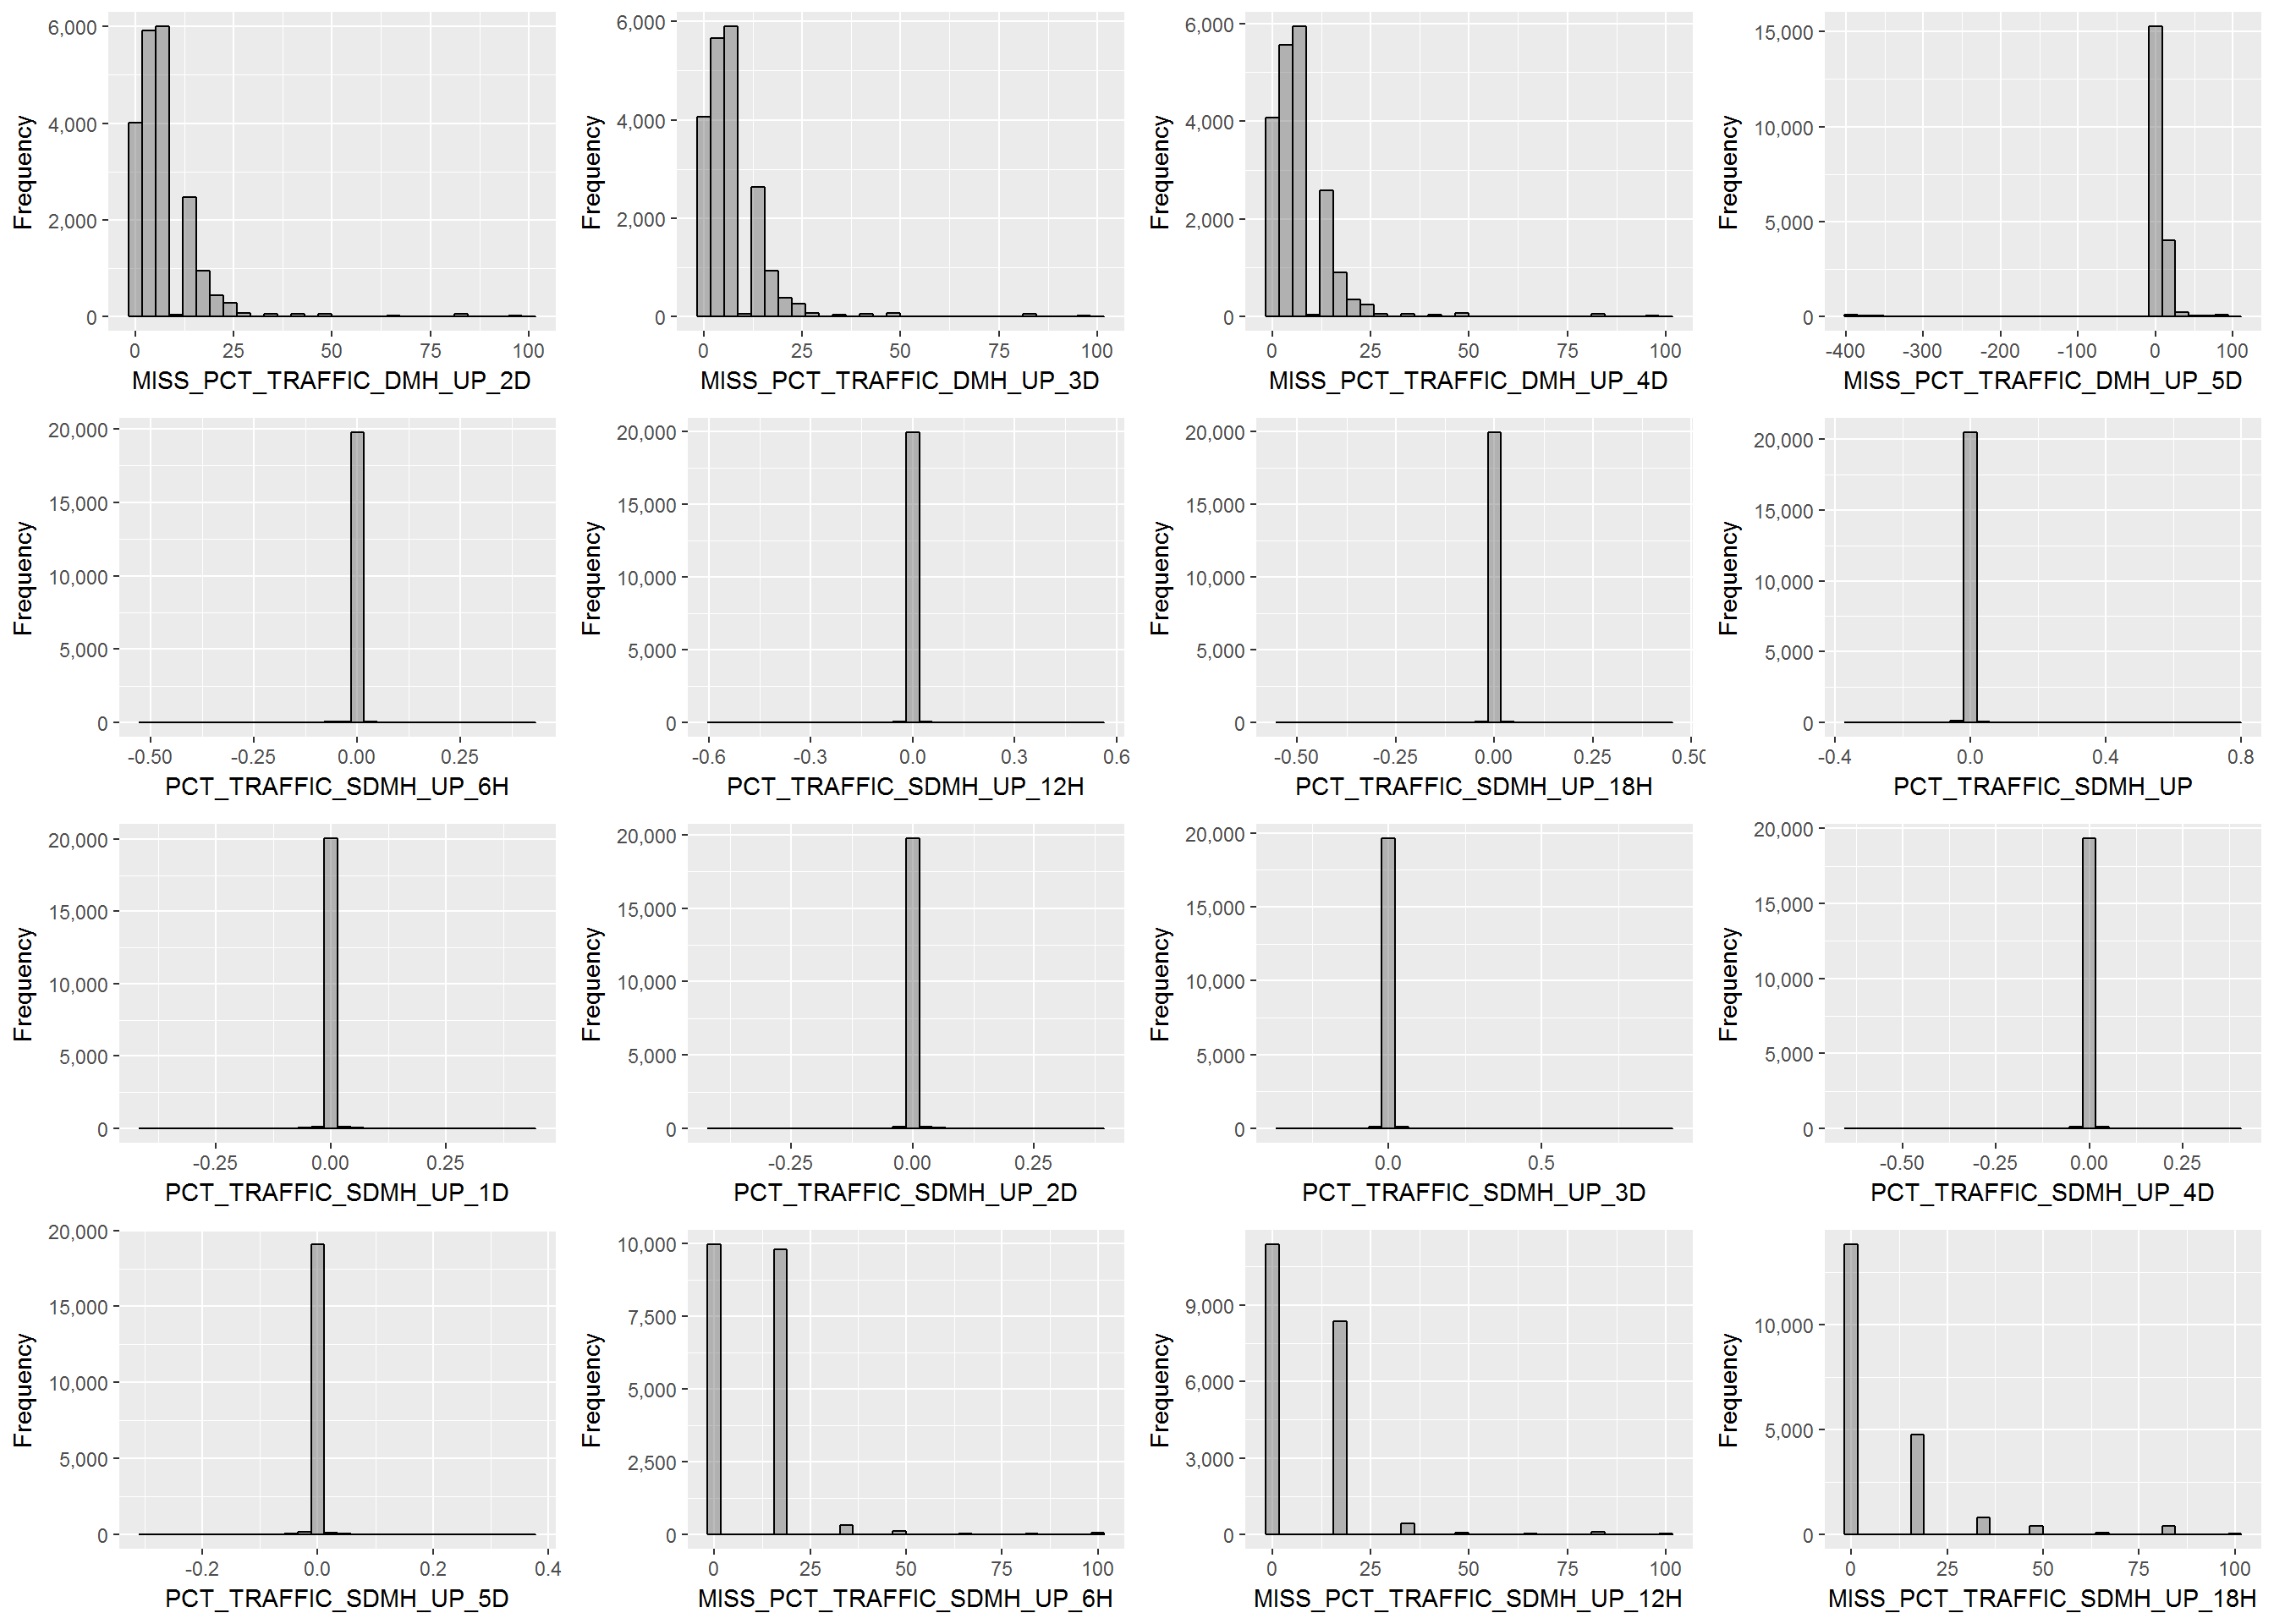
\includegraphics[width=1\linewidth]{continuous-5}
    \end{center}
    \caption{Part 5}
    \label{continuous-5}
\end{figure}

\begin{figure}[ht]
    \begin{center}
    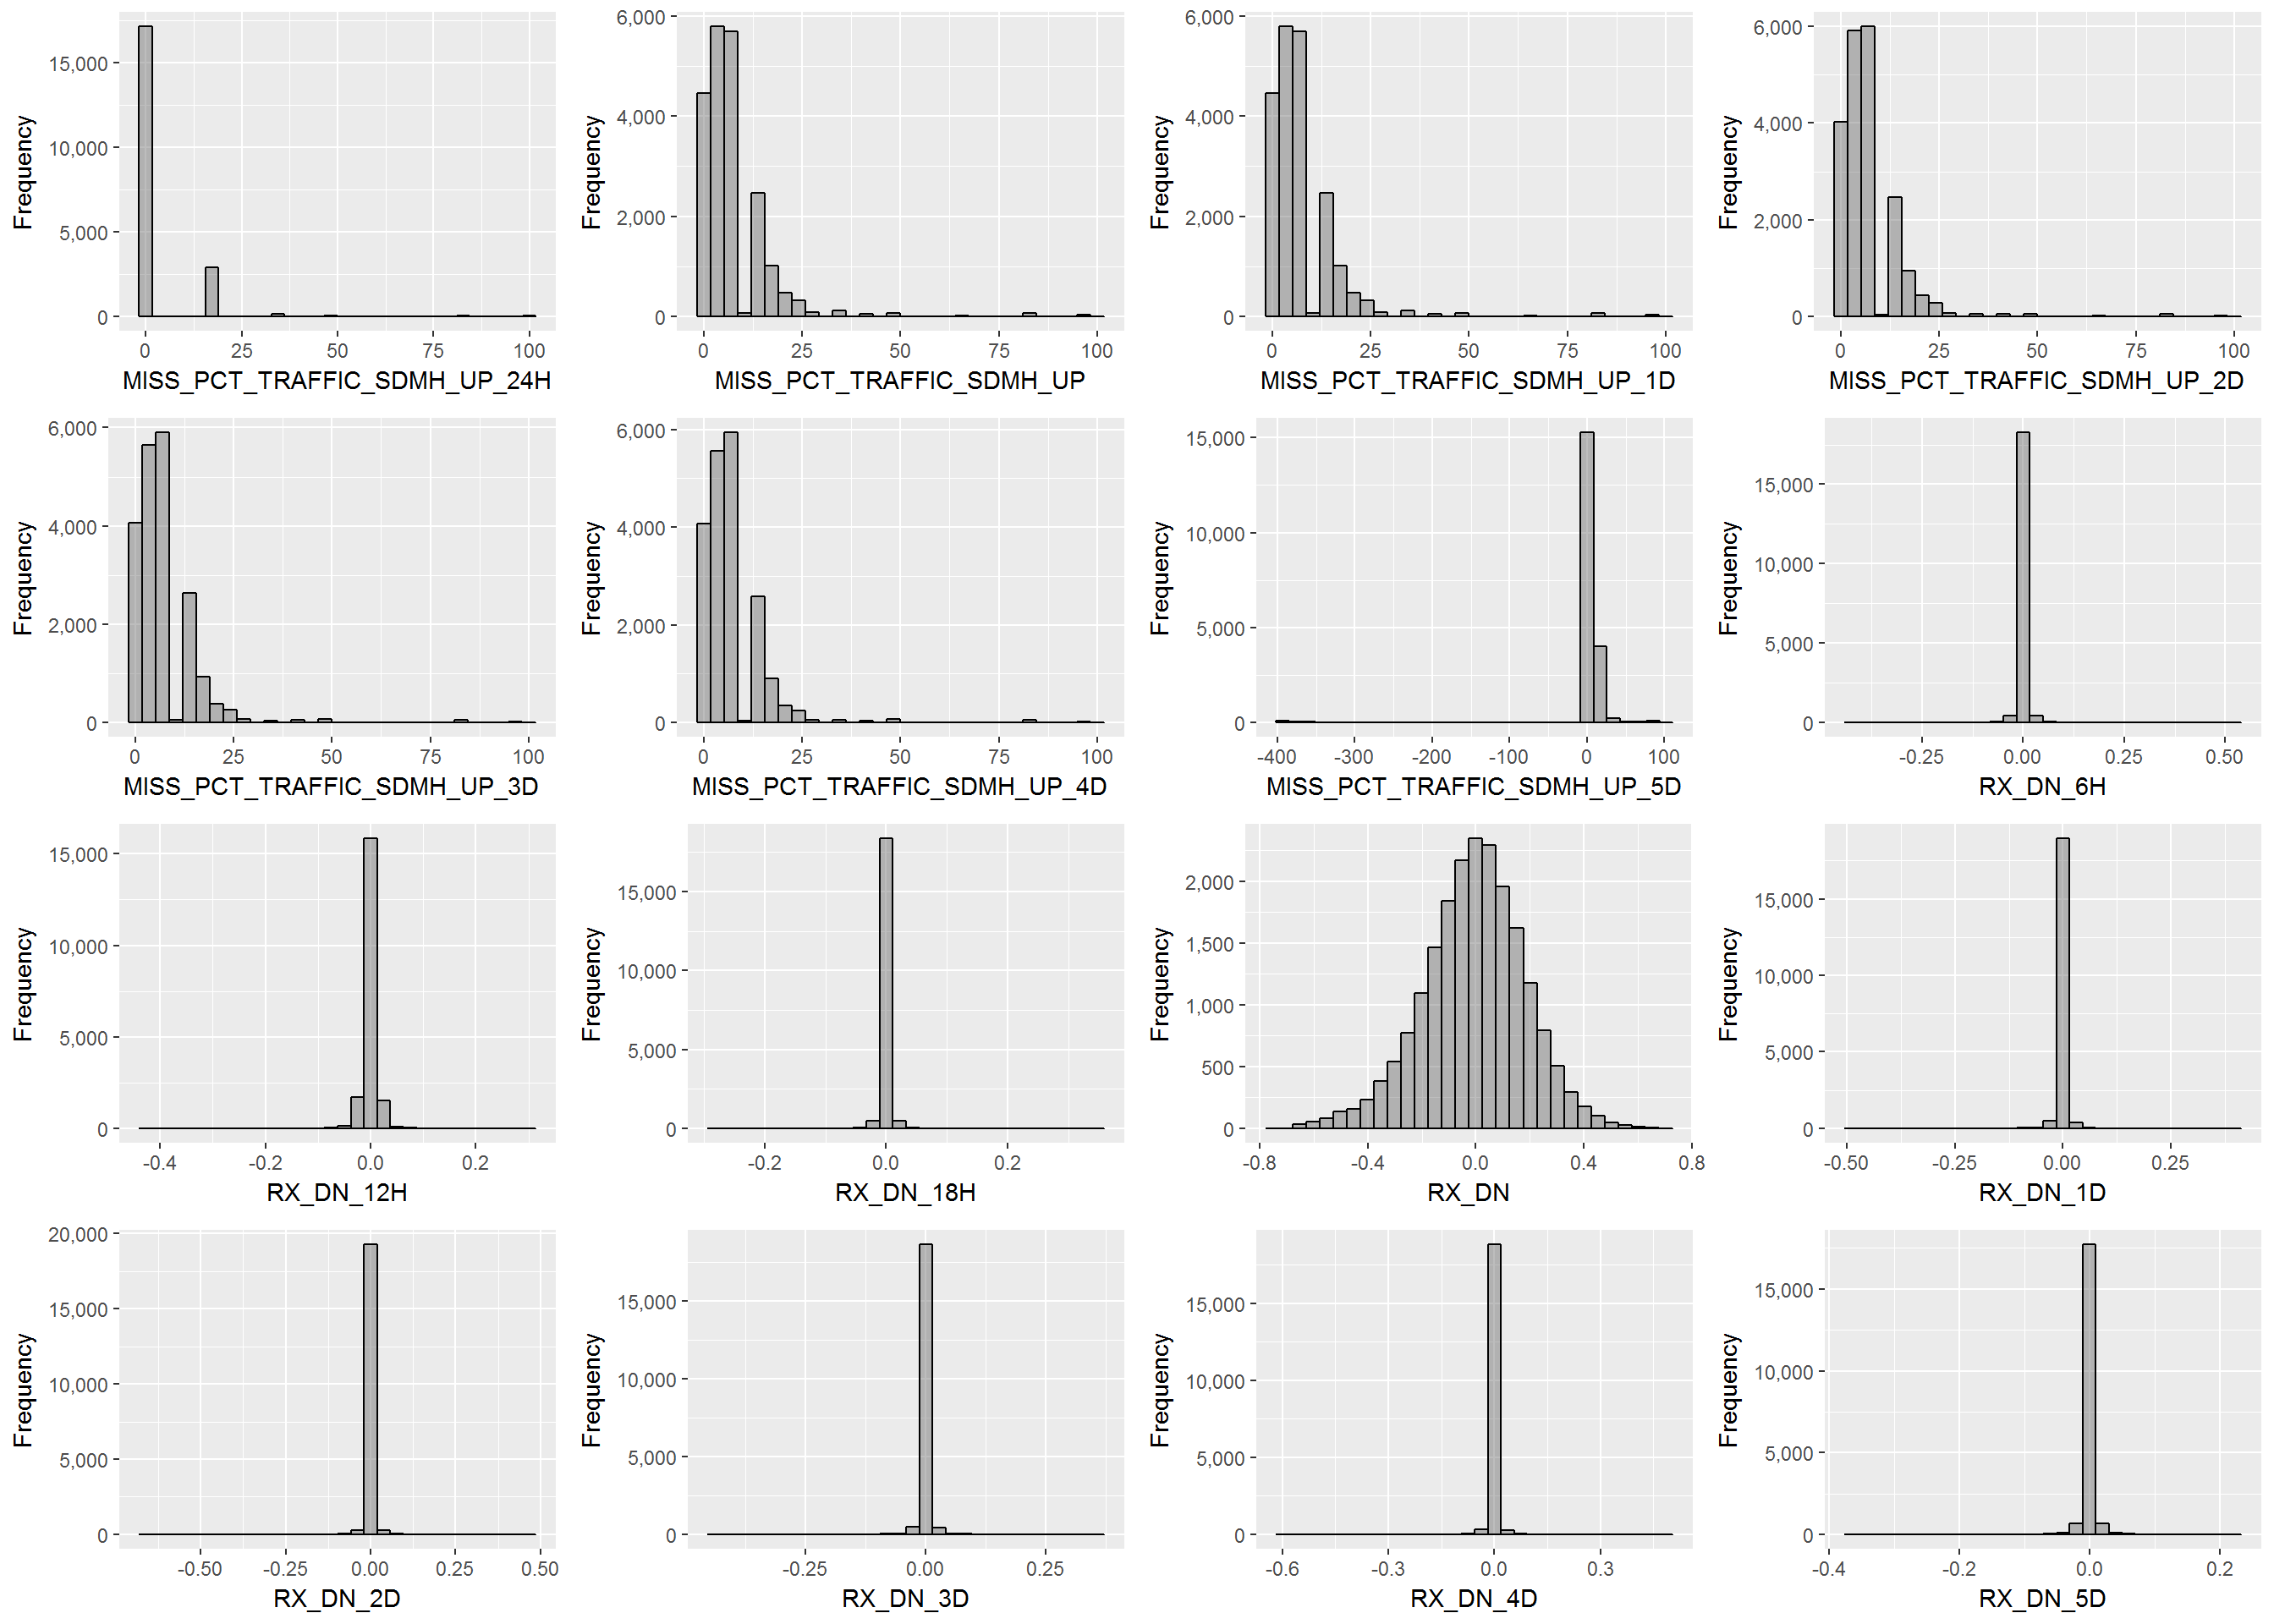
\includegraphics[width=1\linewidth]{continuous-6}
    \end{center}
    \caption{Part 6}
    \label{continuous-6}
\end{figure}

\begin{figure}[ht]
    \begin{center}
    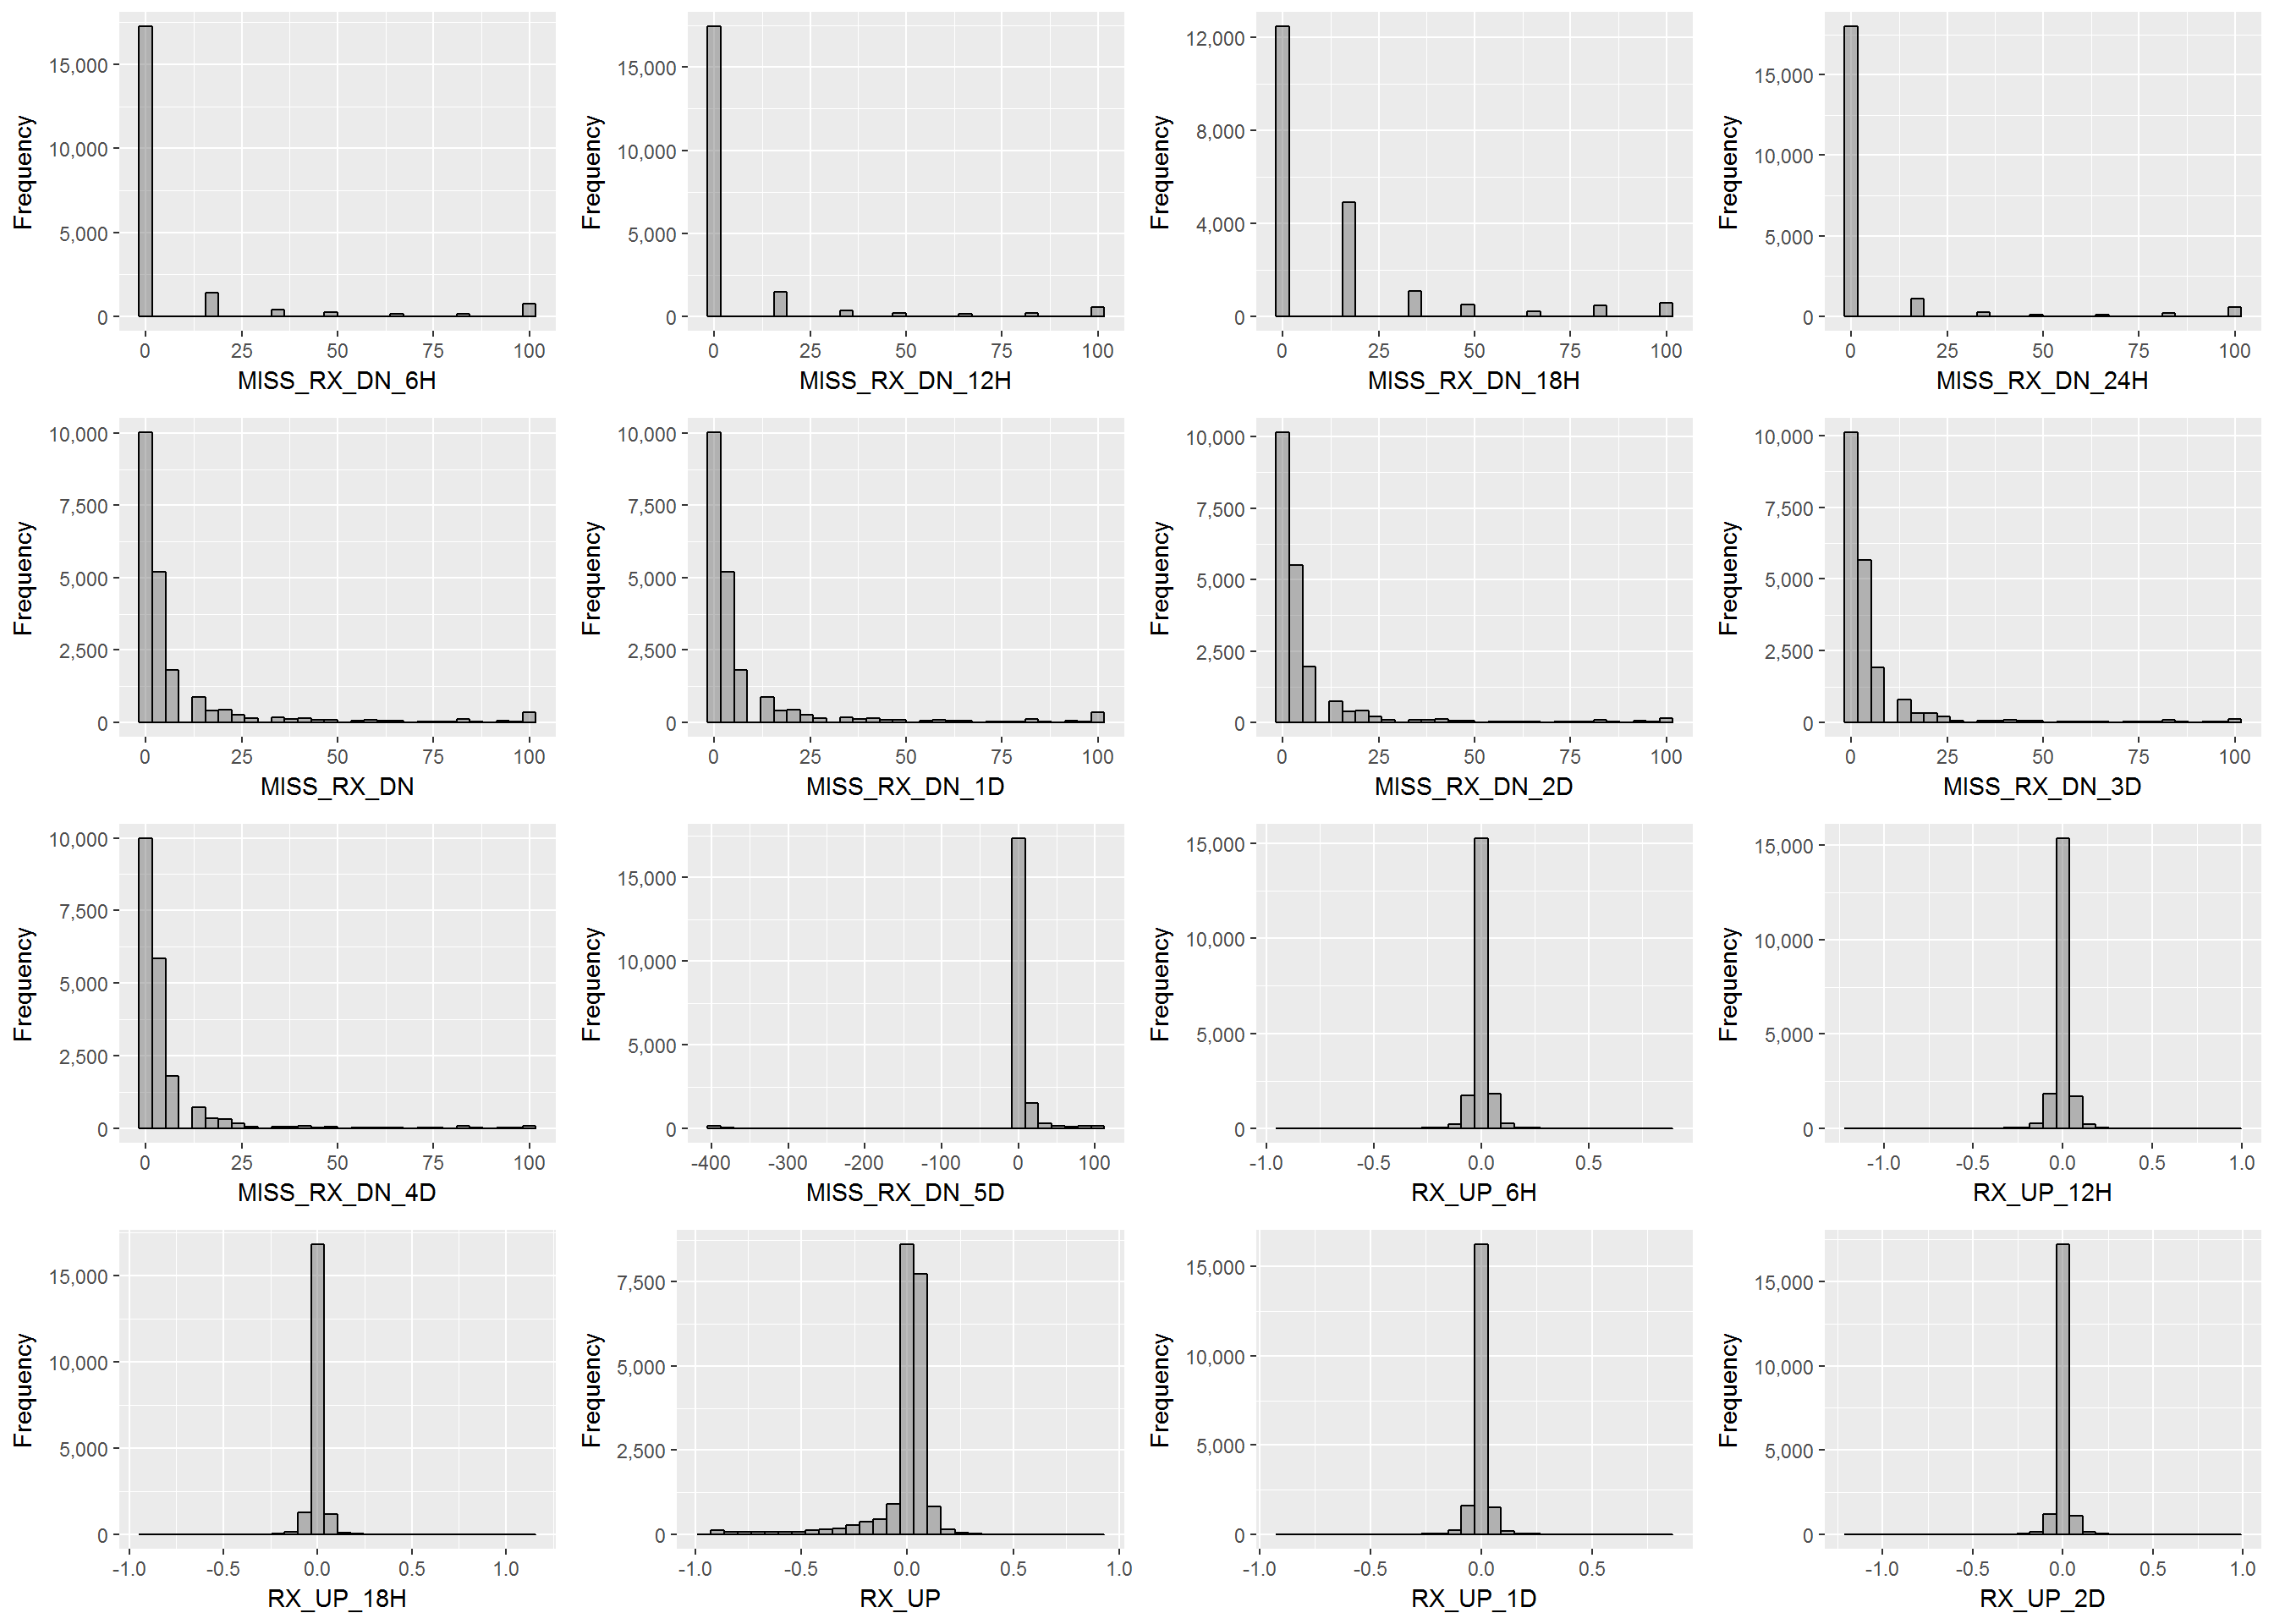
\includegraphics[width=1\linewidth]{continuous-7}
    \end{center}
    \caption{Part 7}
    \label{continuous-7}
\end{figure}

\begin{figure}[ht]
    \begin{center}
    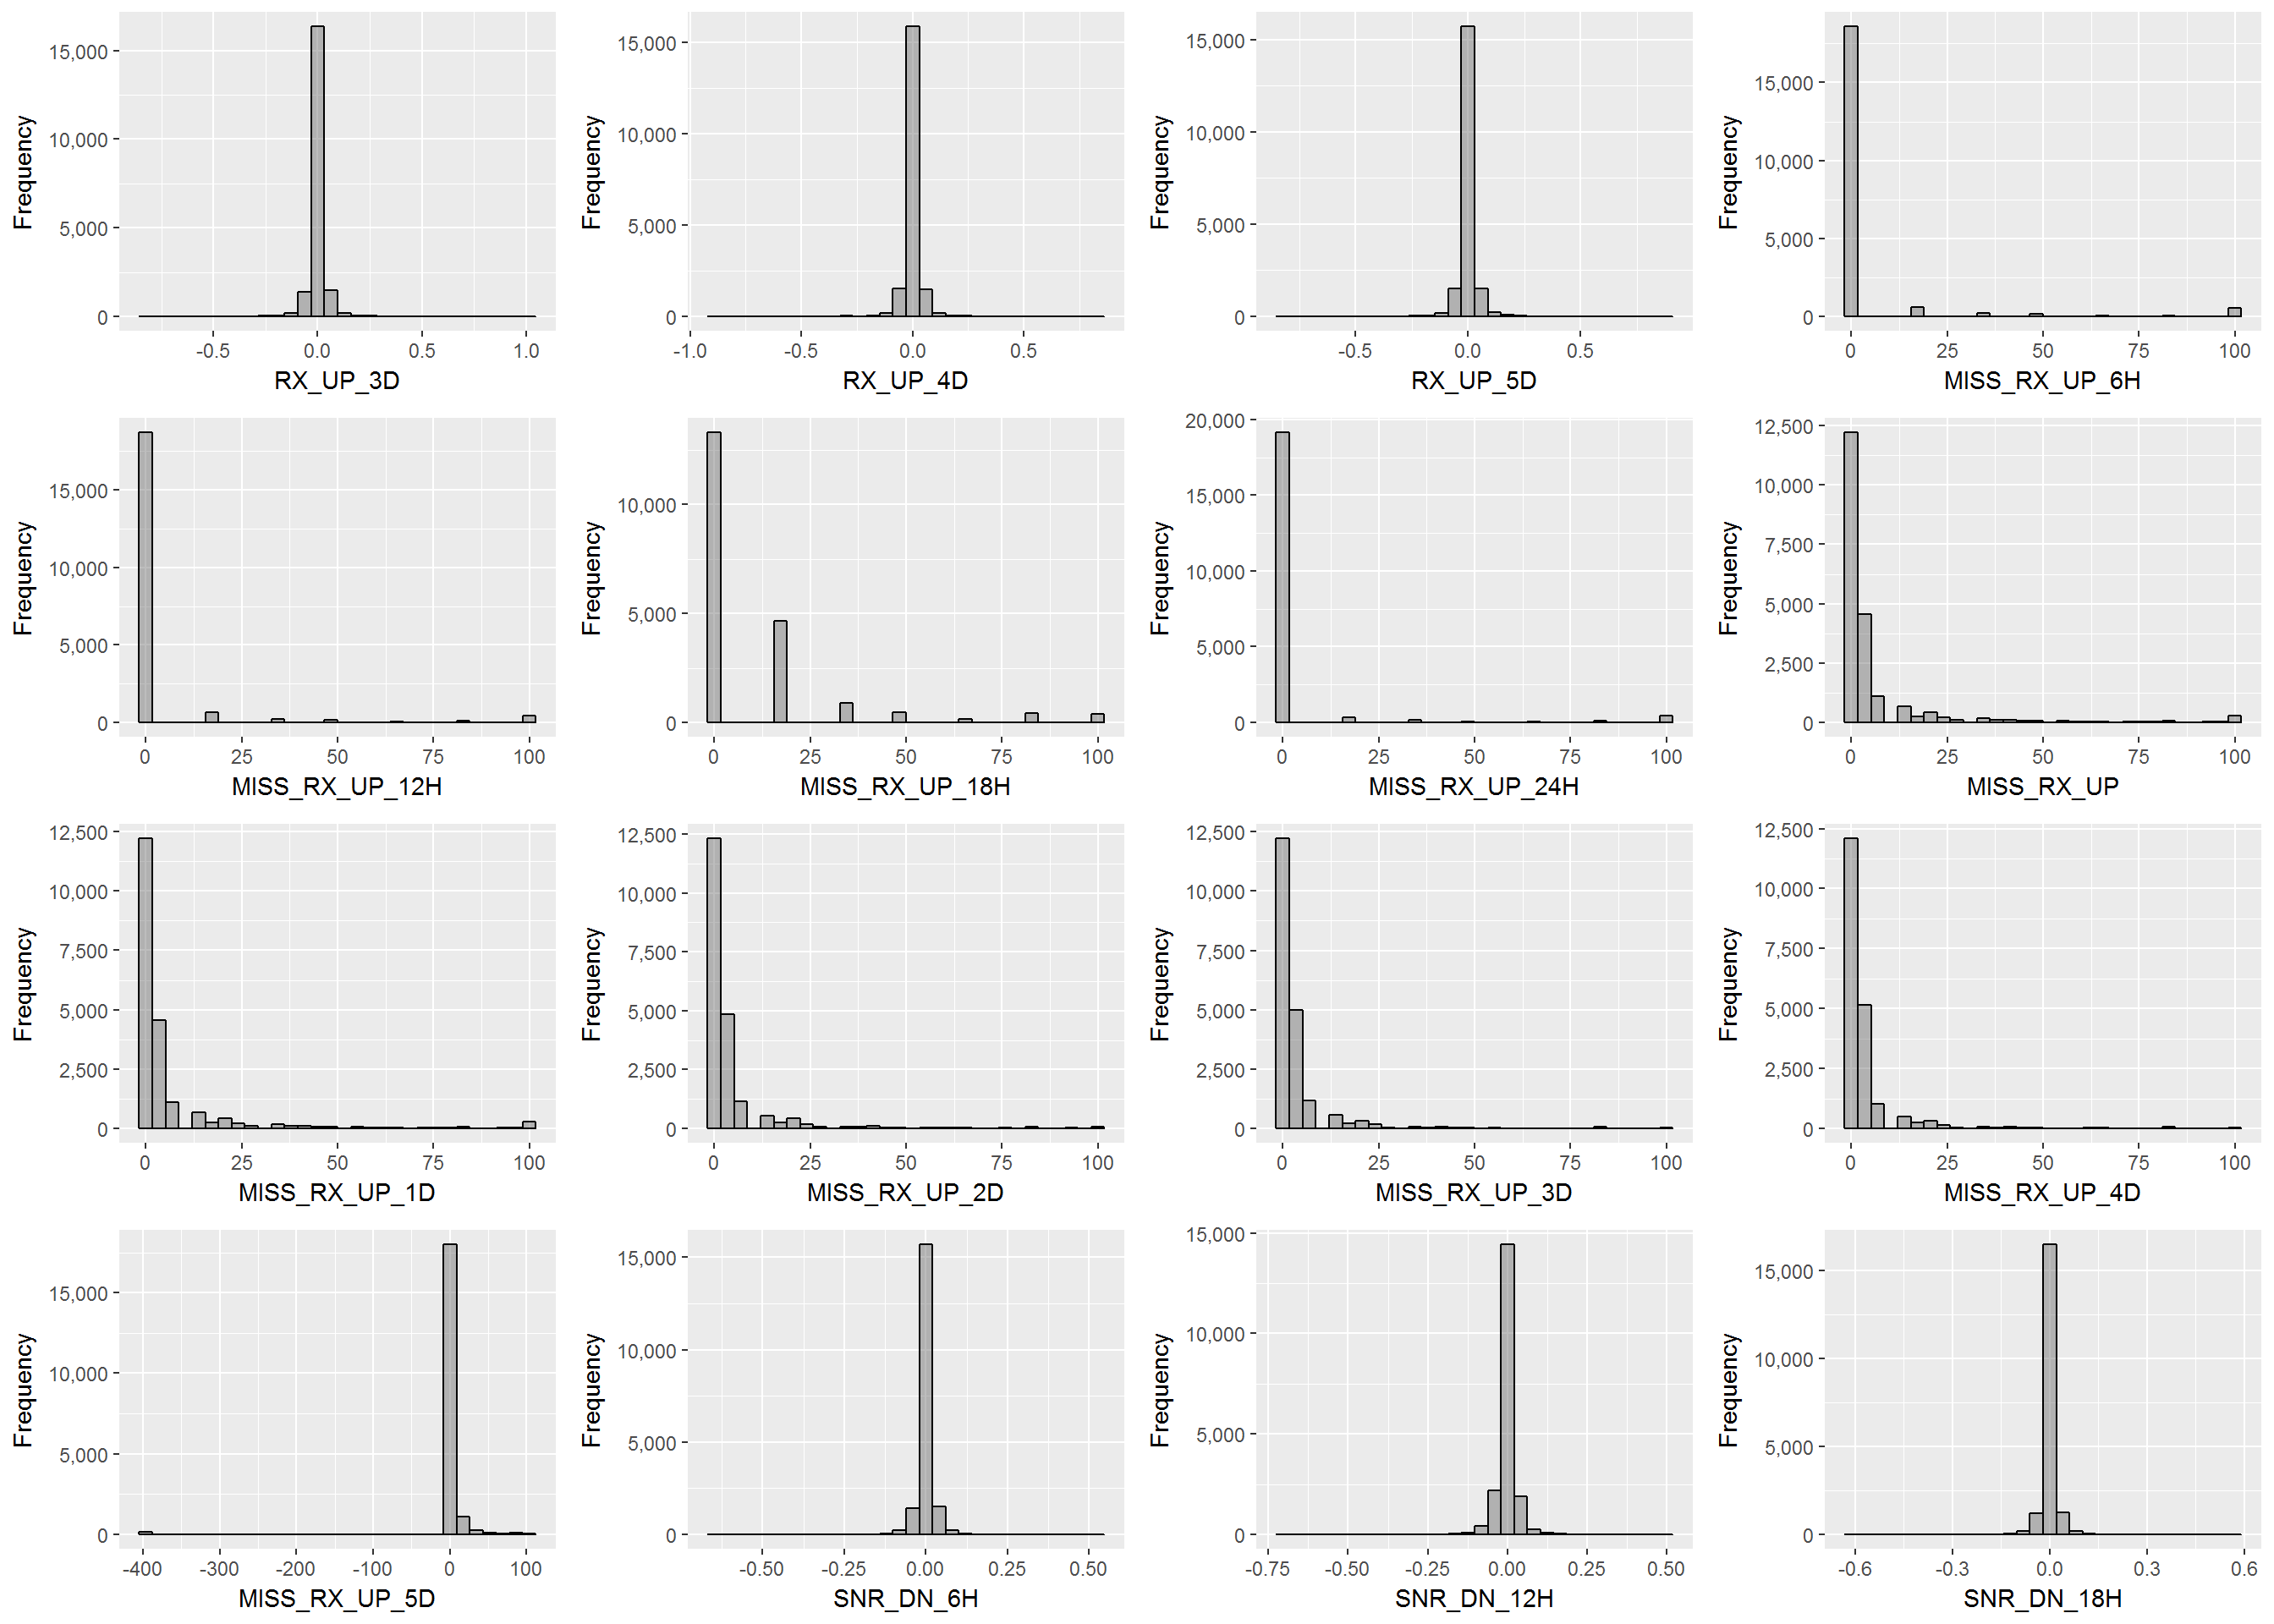
\includegraphics[width=1\linewidth]{continuous-8}
    \end{center}
    \caption{Part 8}
    \label{continuous-8}
\end{figure}

\begin{figure}[ht]
    \begin{center}
    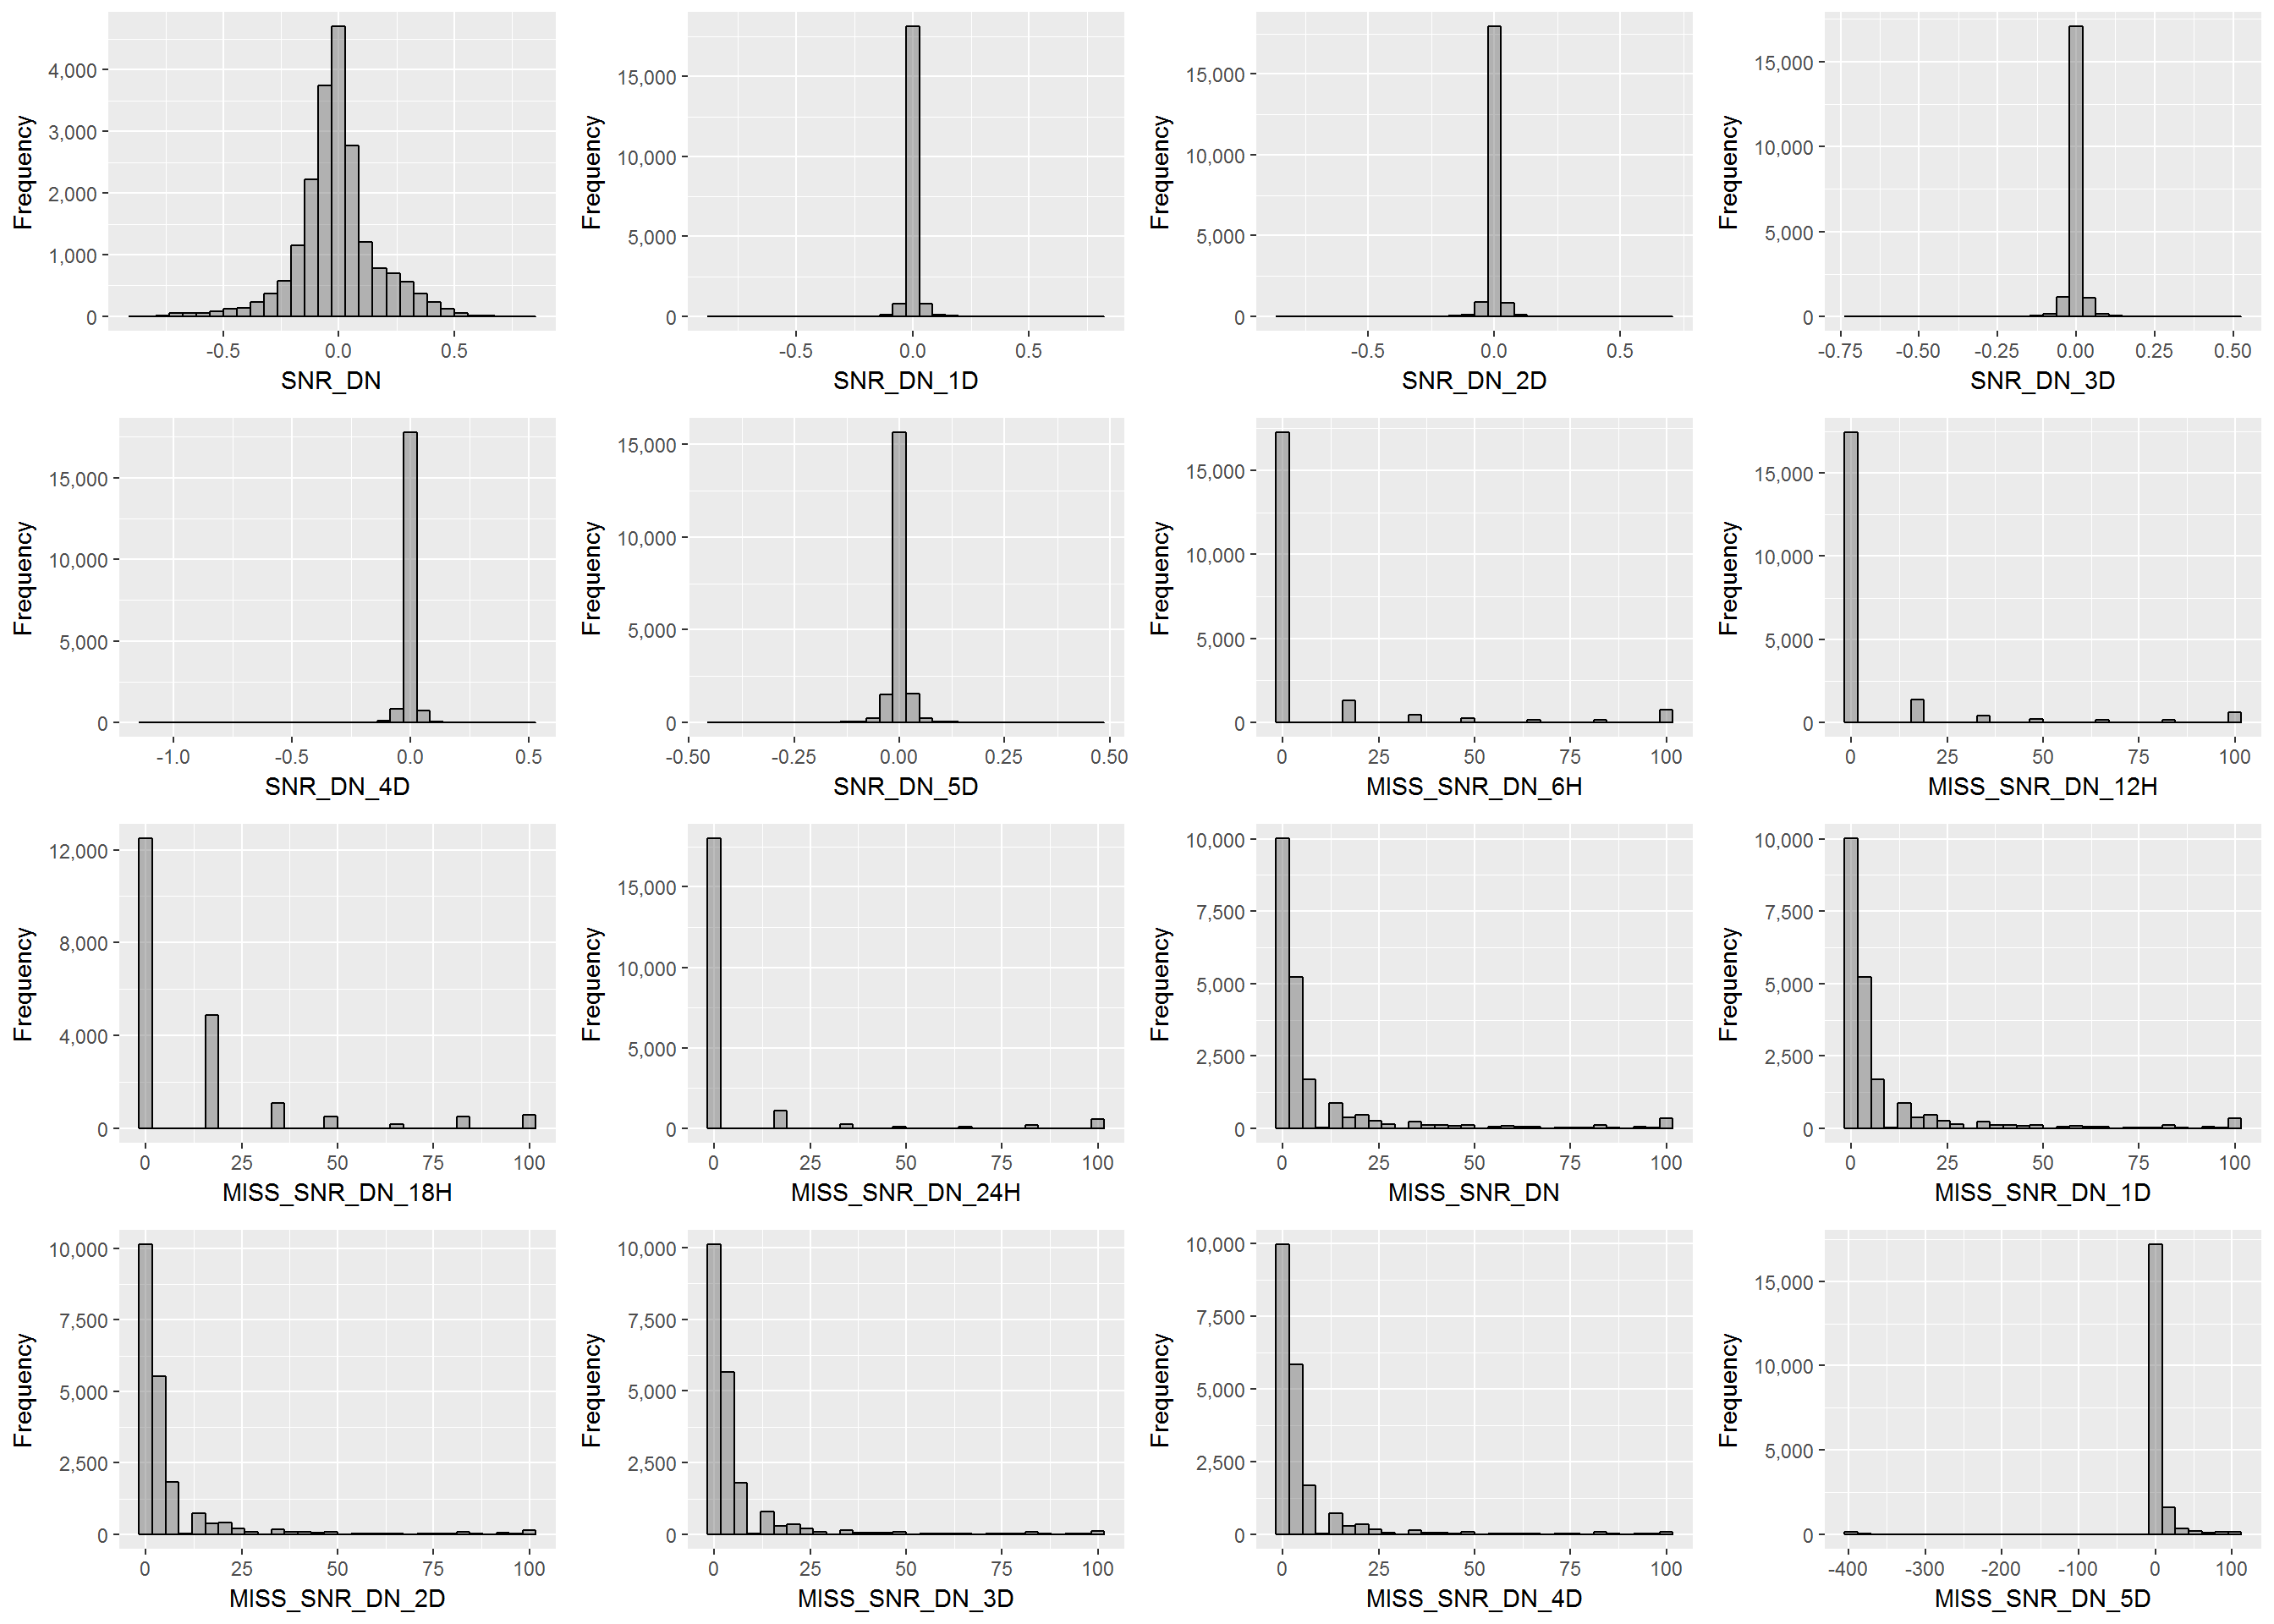
\includegraphics[width=1\linewidth]{continuous-9}
    \end{center}
    \caption{Part 9}
    \label{continuous-9}
\end{figure}

\begin{figure}[ht]
    \begin{center}
    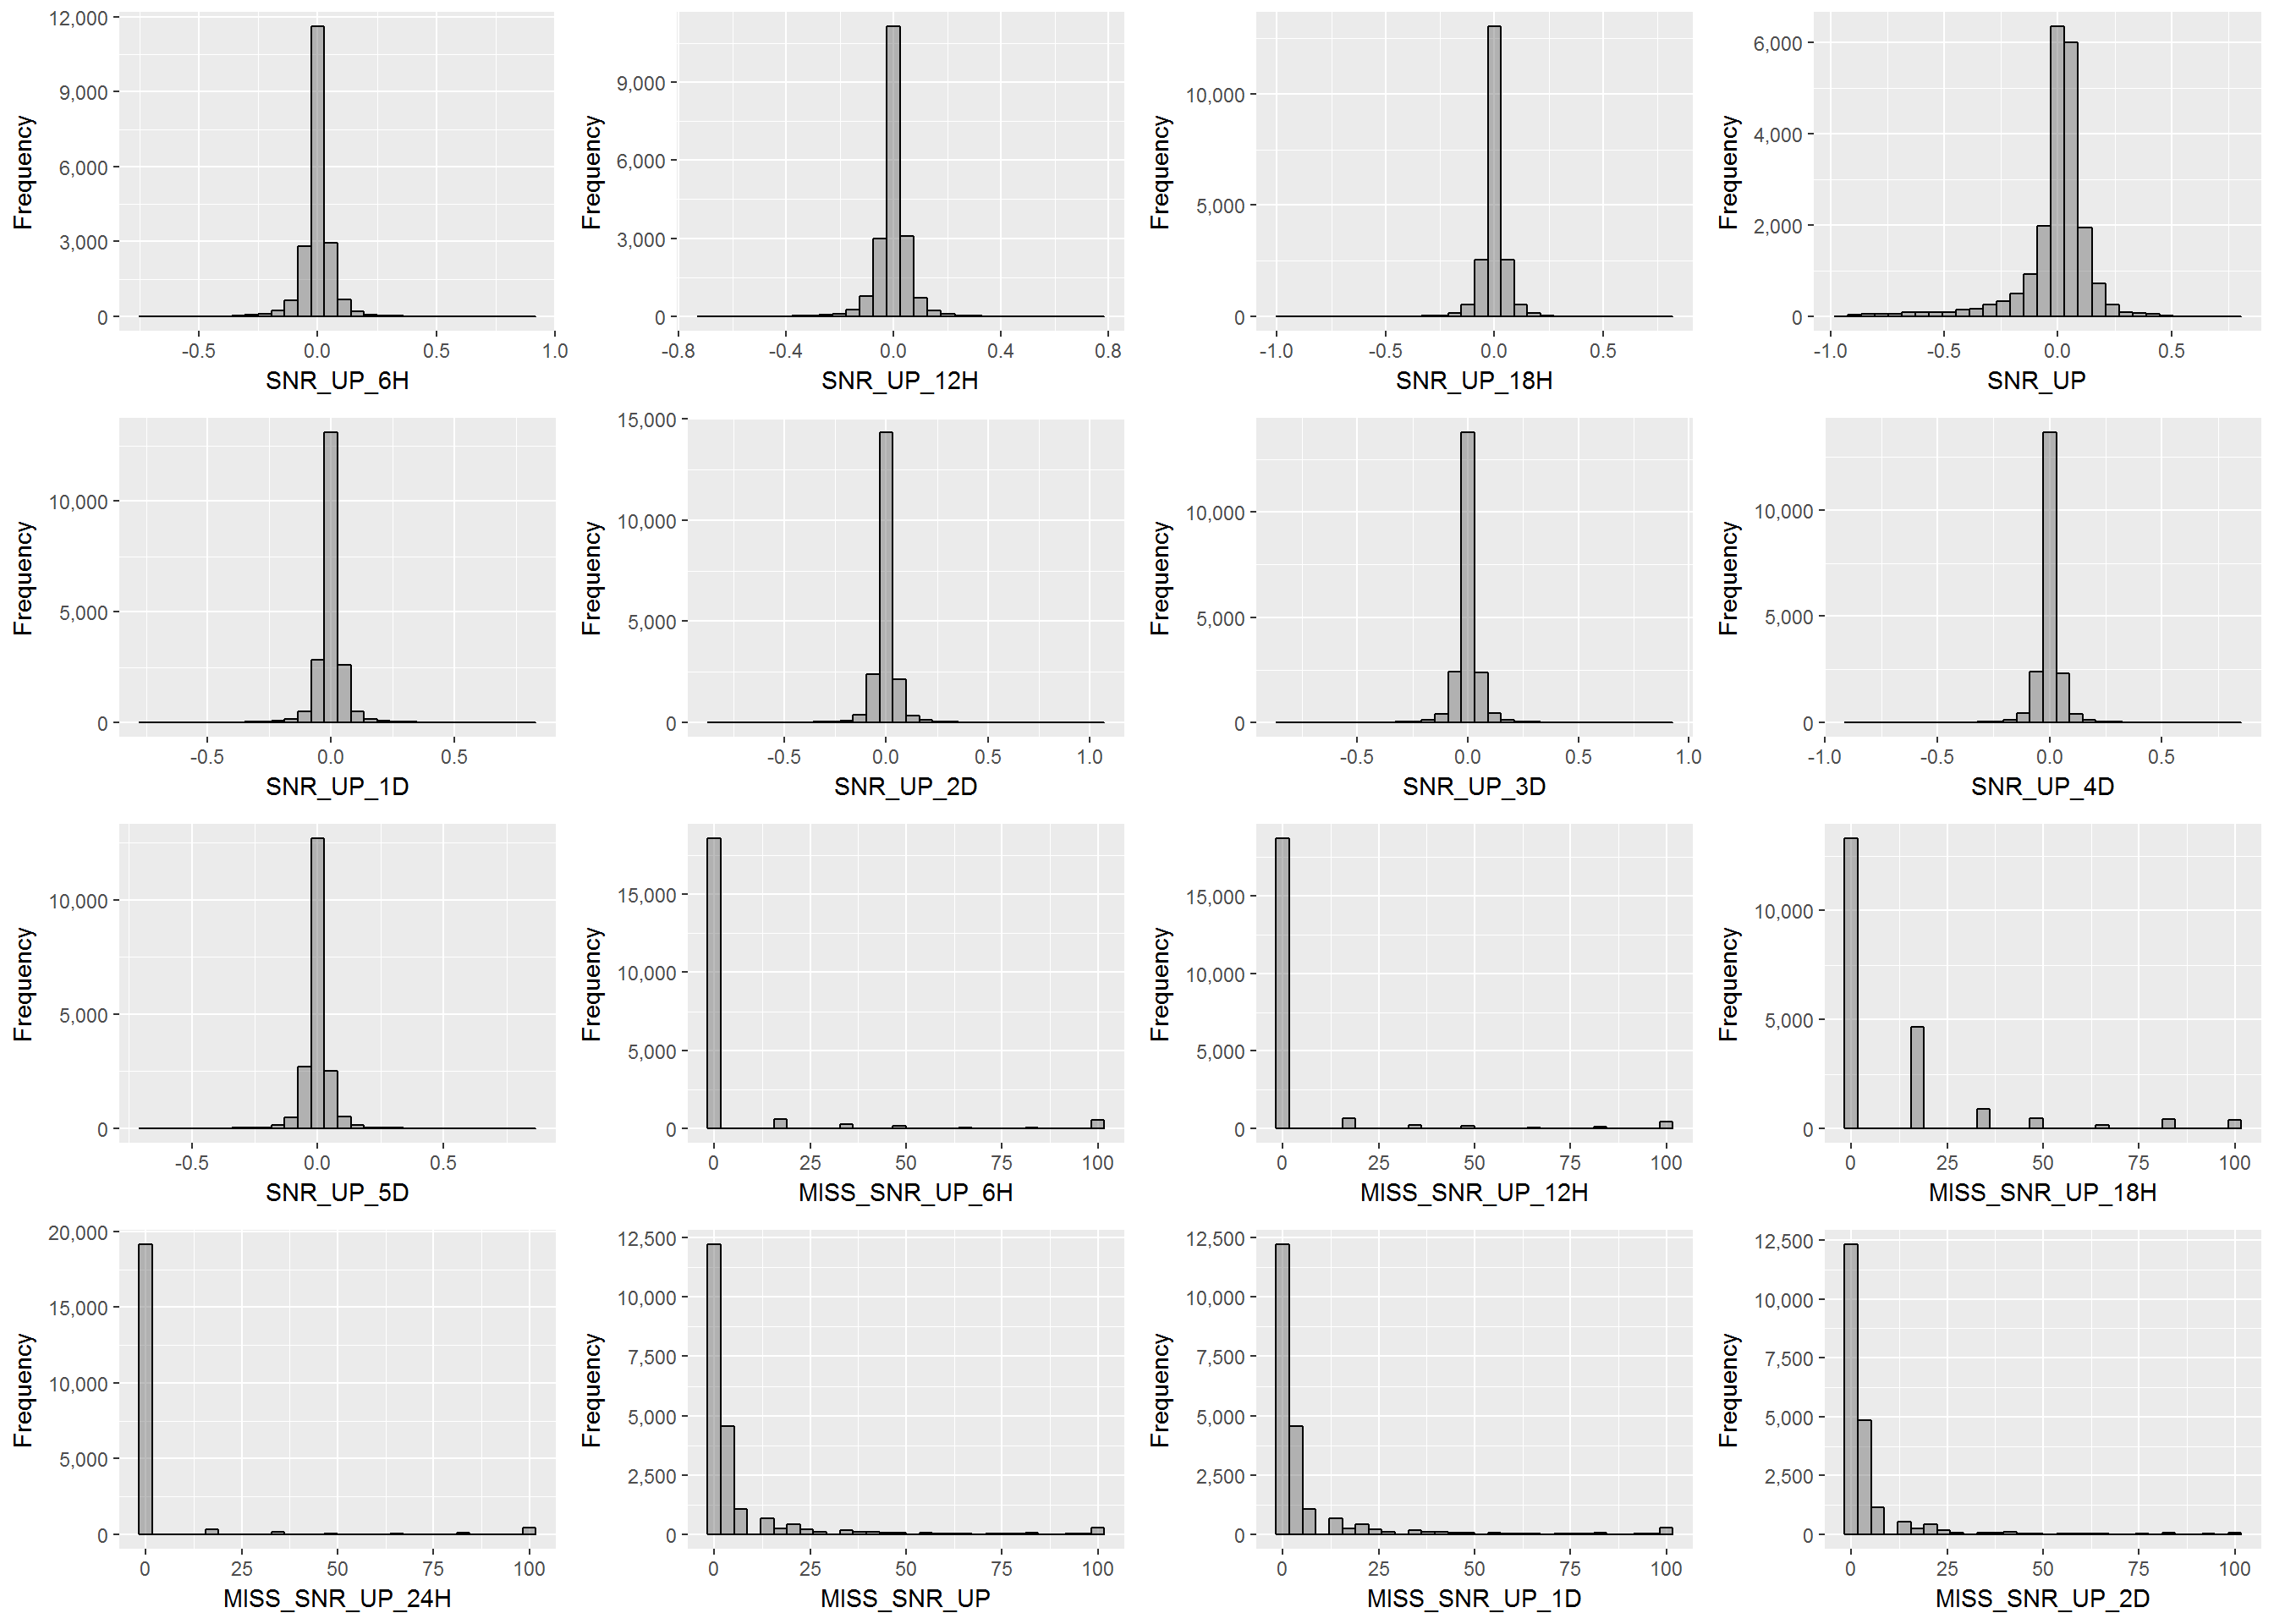
\includegraphics[width=1\linewidth]{continuous-10}
    \end{center}
    \caption{Part 10}
    \label{continuous-10}
\end{figure}

\begin{figure}[ht]
    \begin{center}
    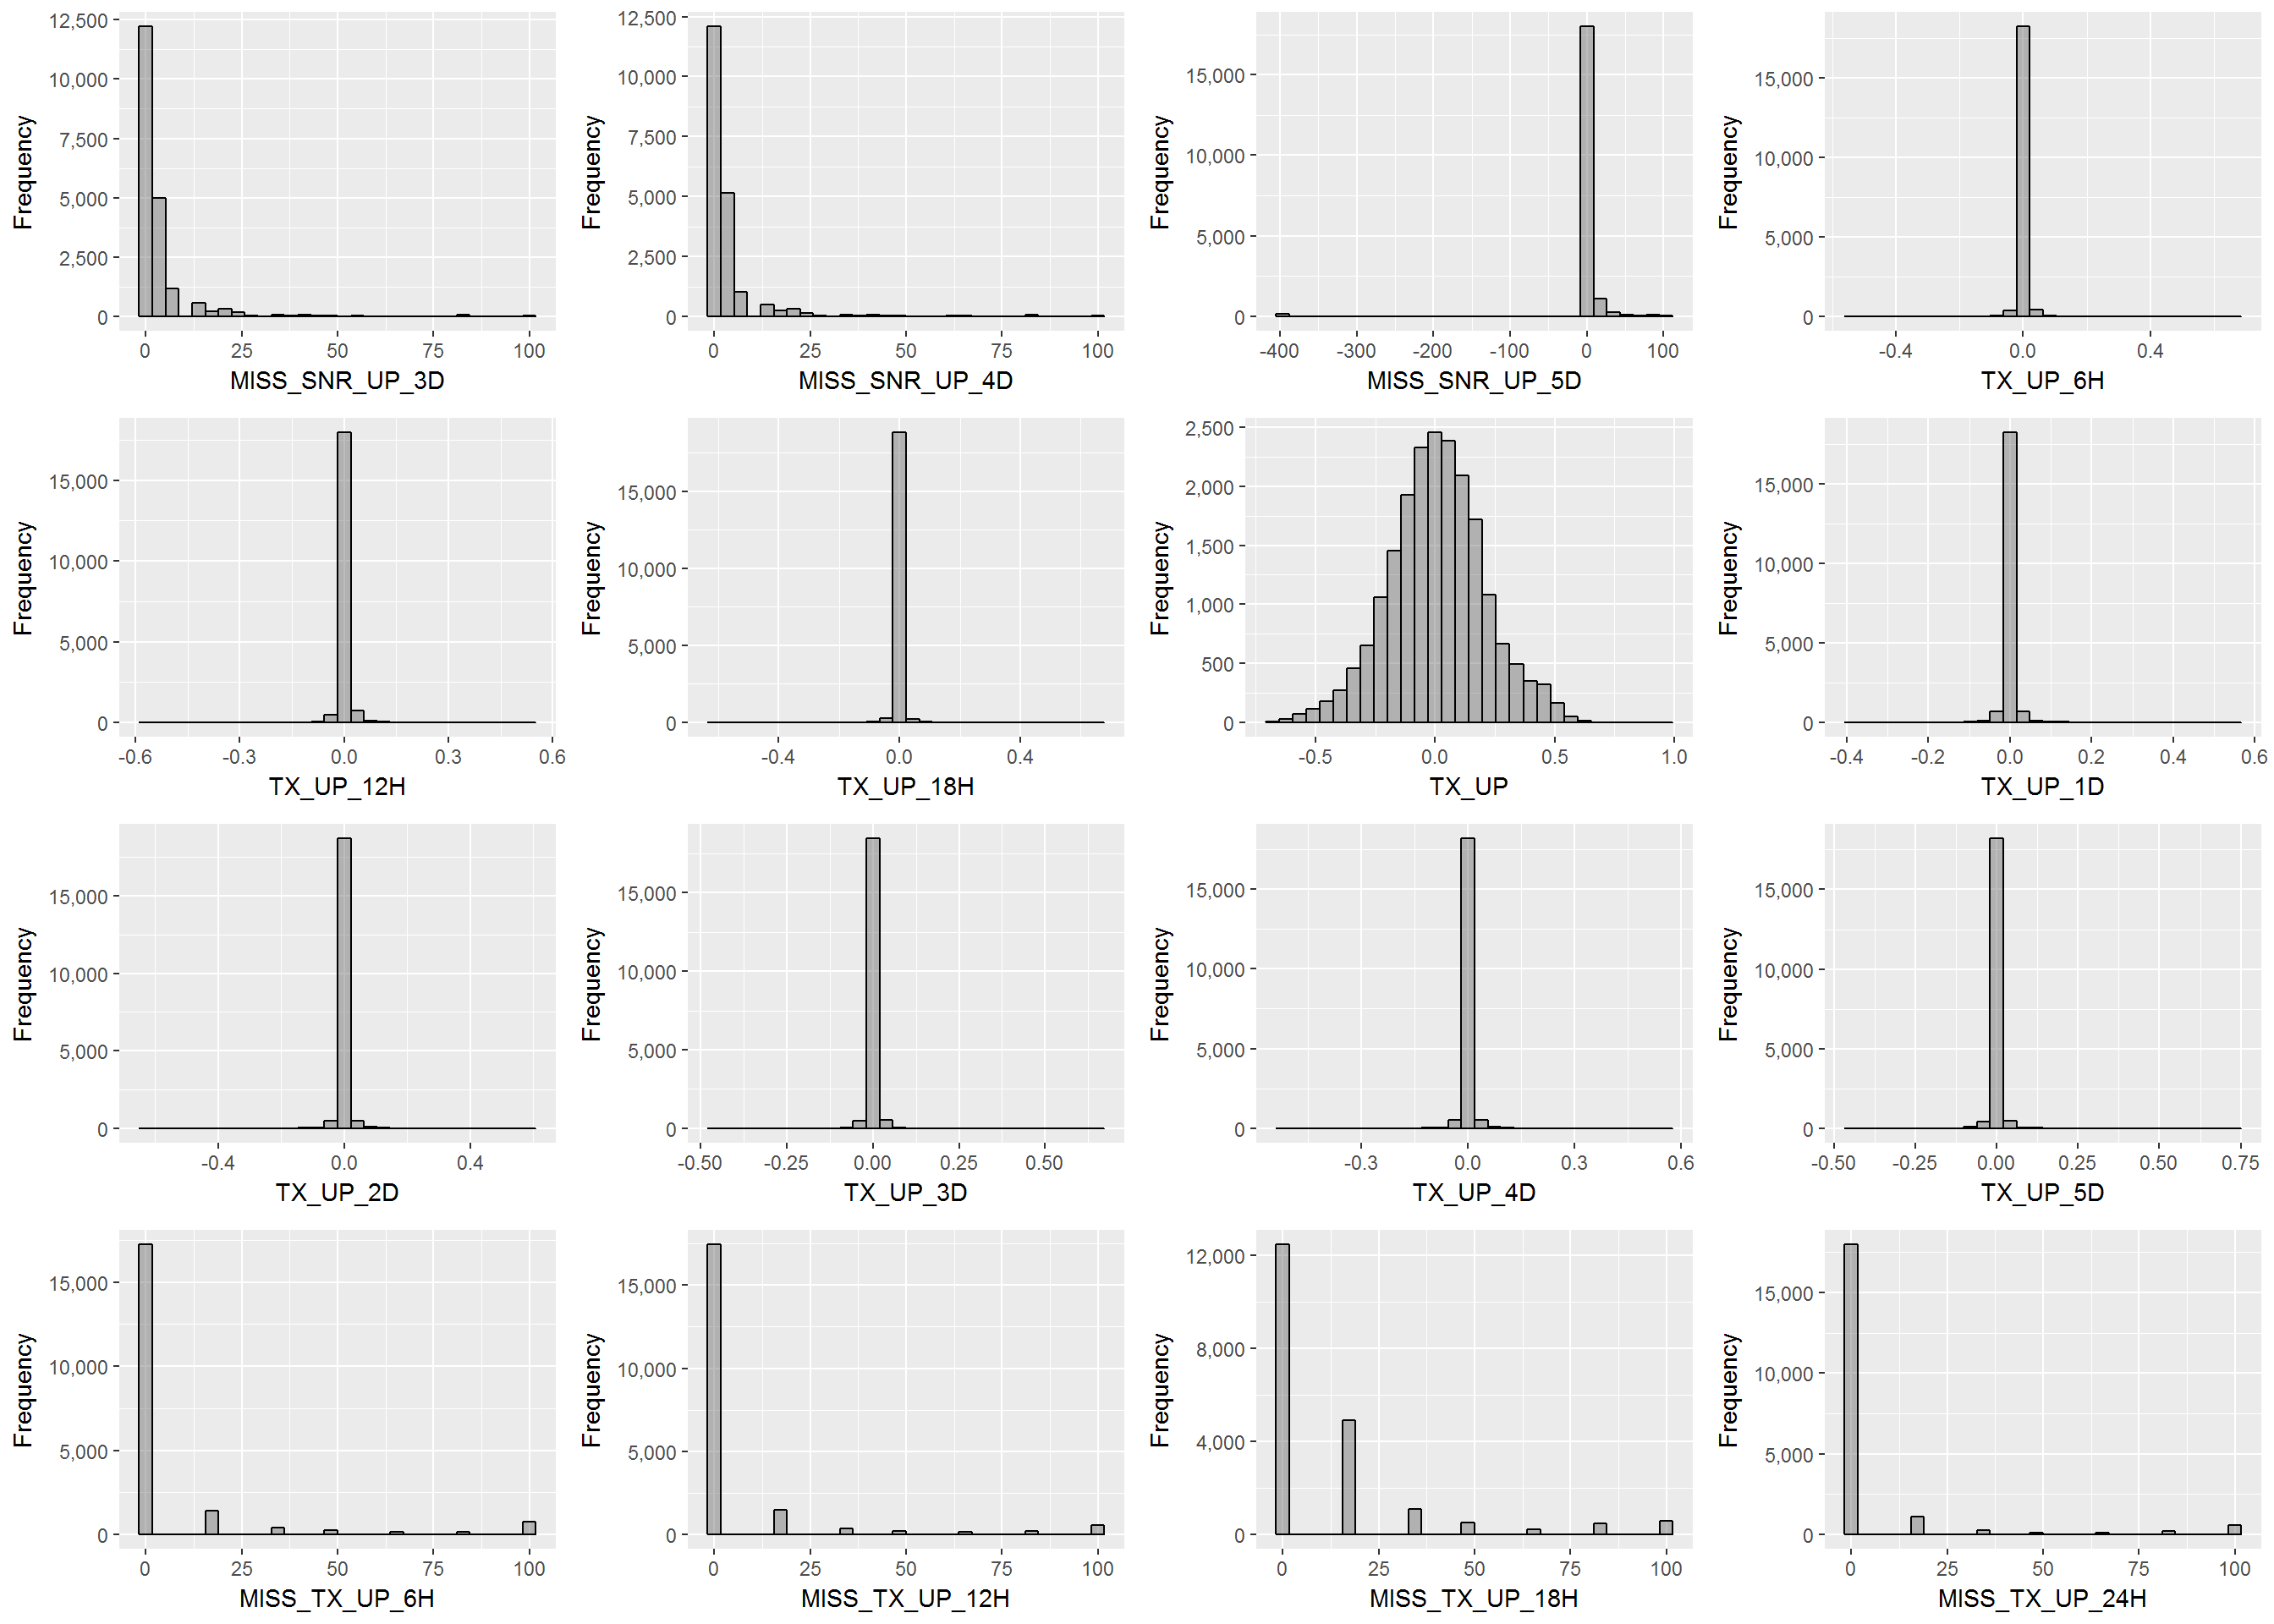
\includegraphics[width=1\linewidth]{continuous-11}
    \end{center}
    \caption{Part 11}
    \label{continuous-11}
\end{figure}

\begin{figure}[ht]
    \begin{center}
    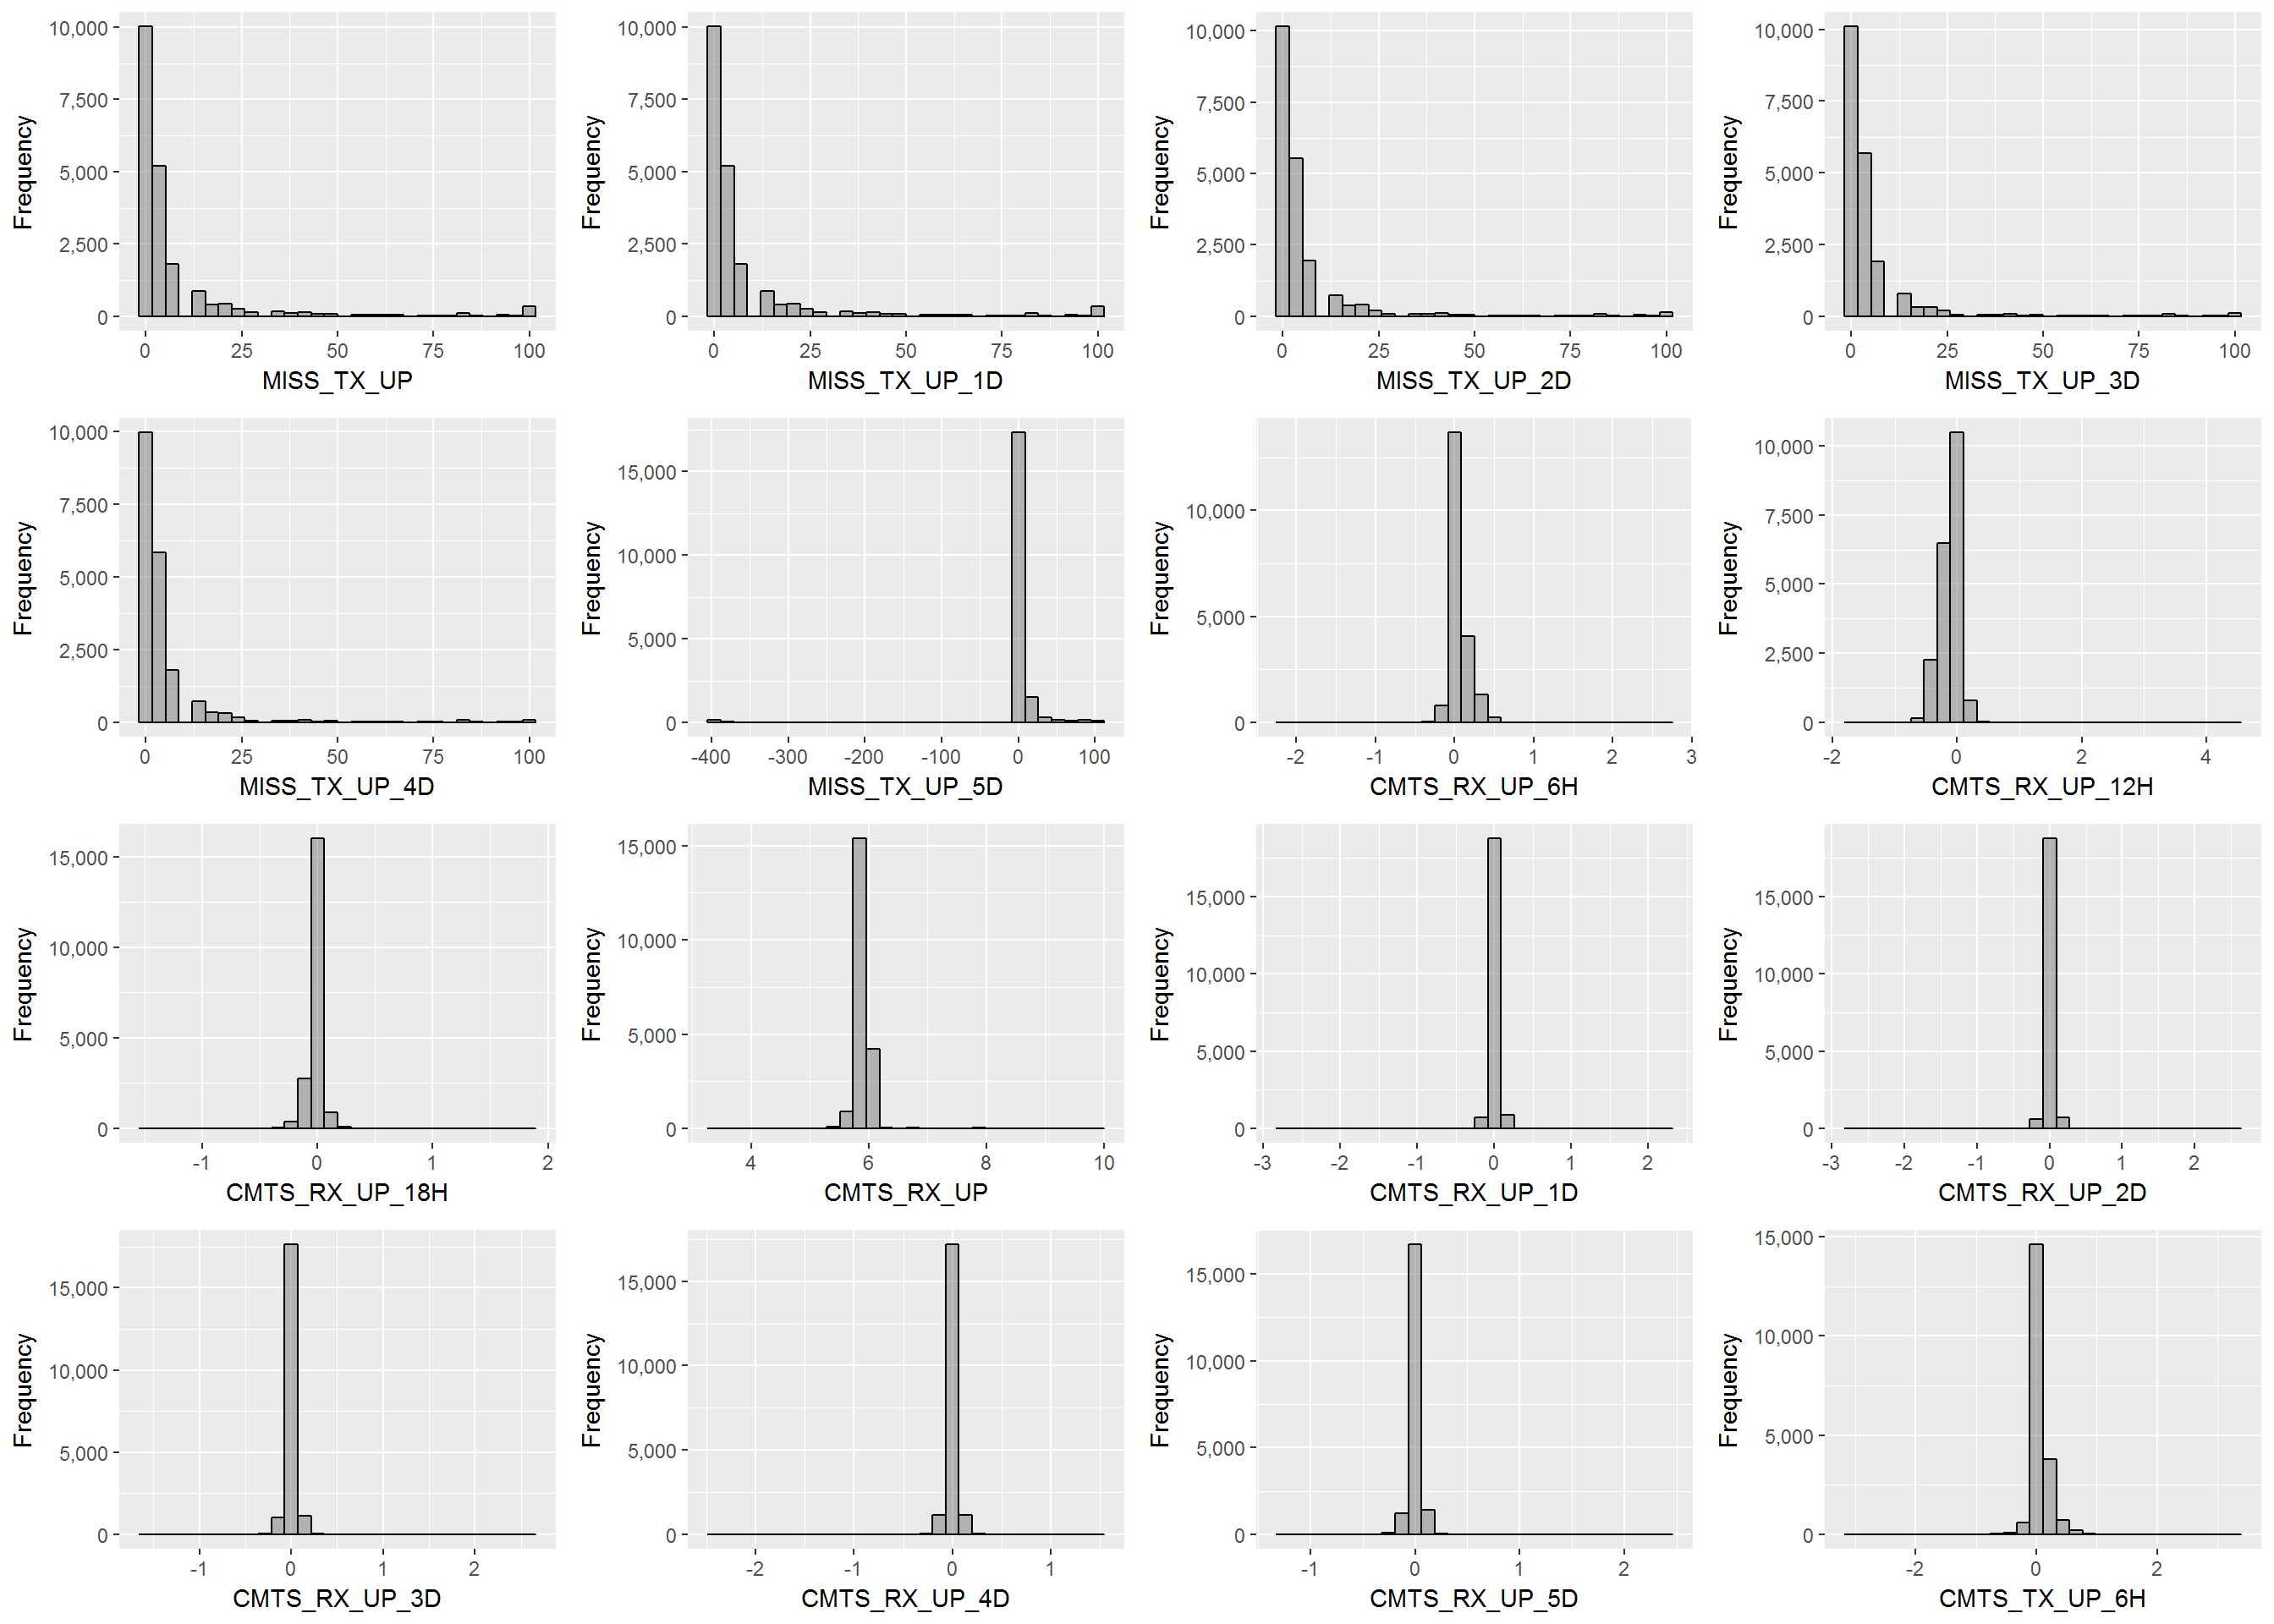
\includegraphics[width=1\linewidth]{continuous-12}
    \end{center}
    \caption{Part 12}
    \label{continuous-12}
\end{figure}

\begin{figure}[ht]
    \begin{center}
    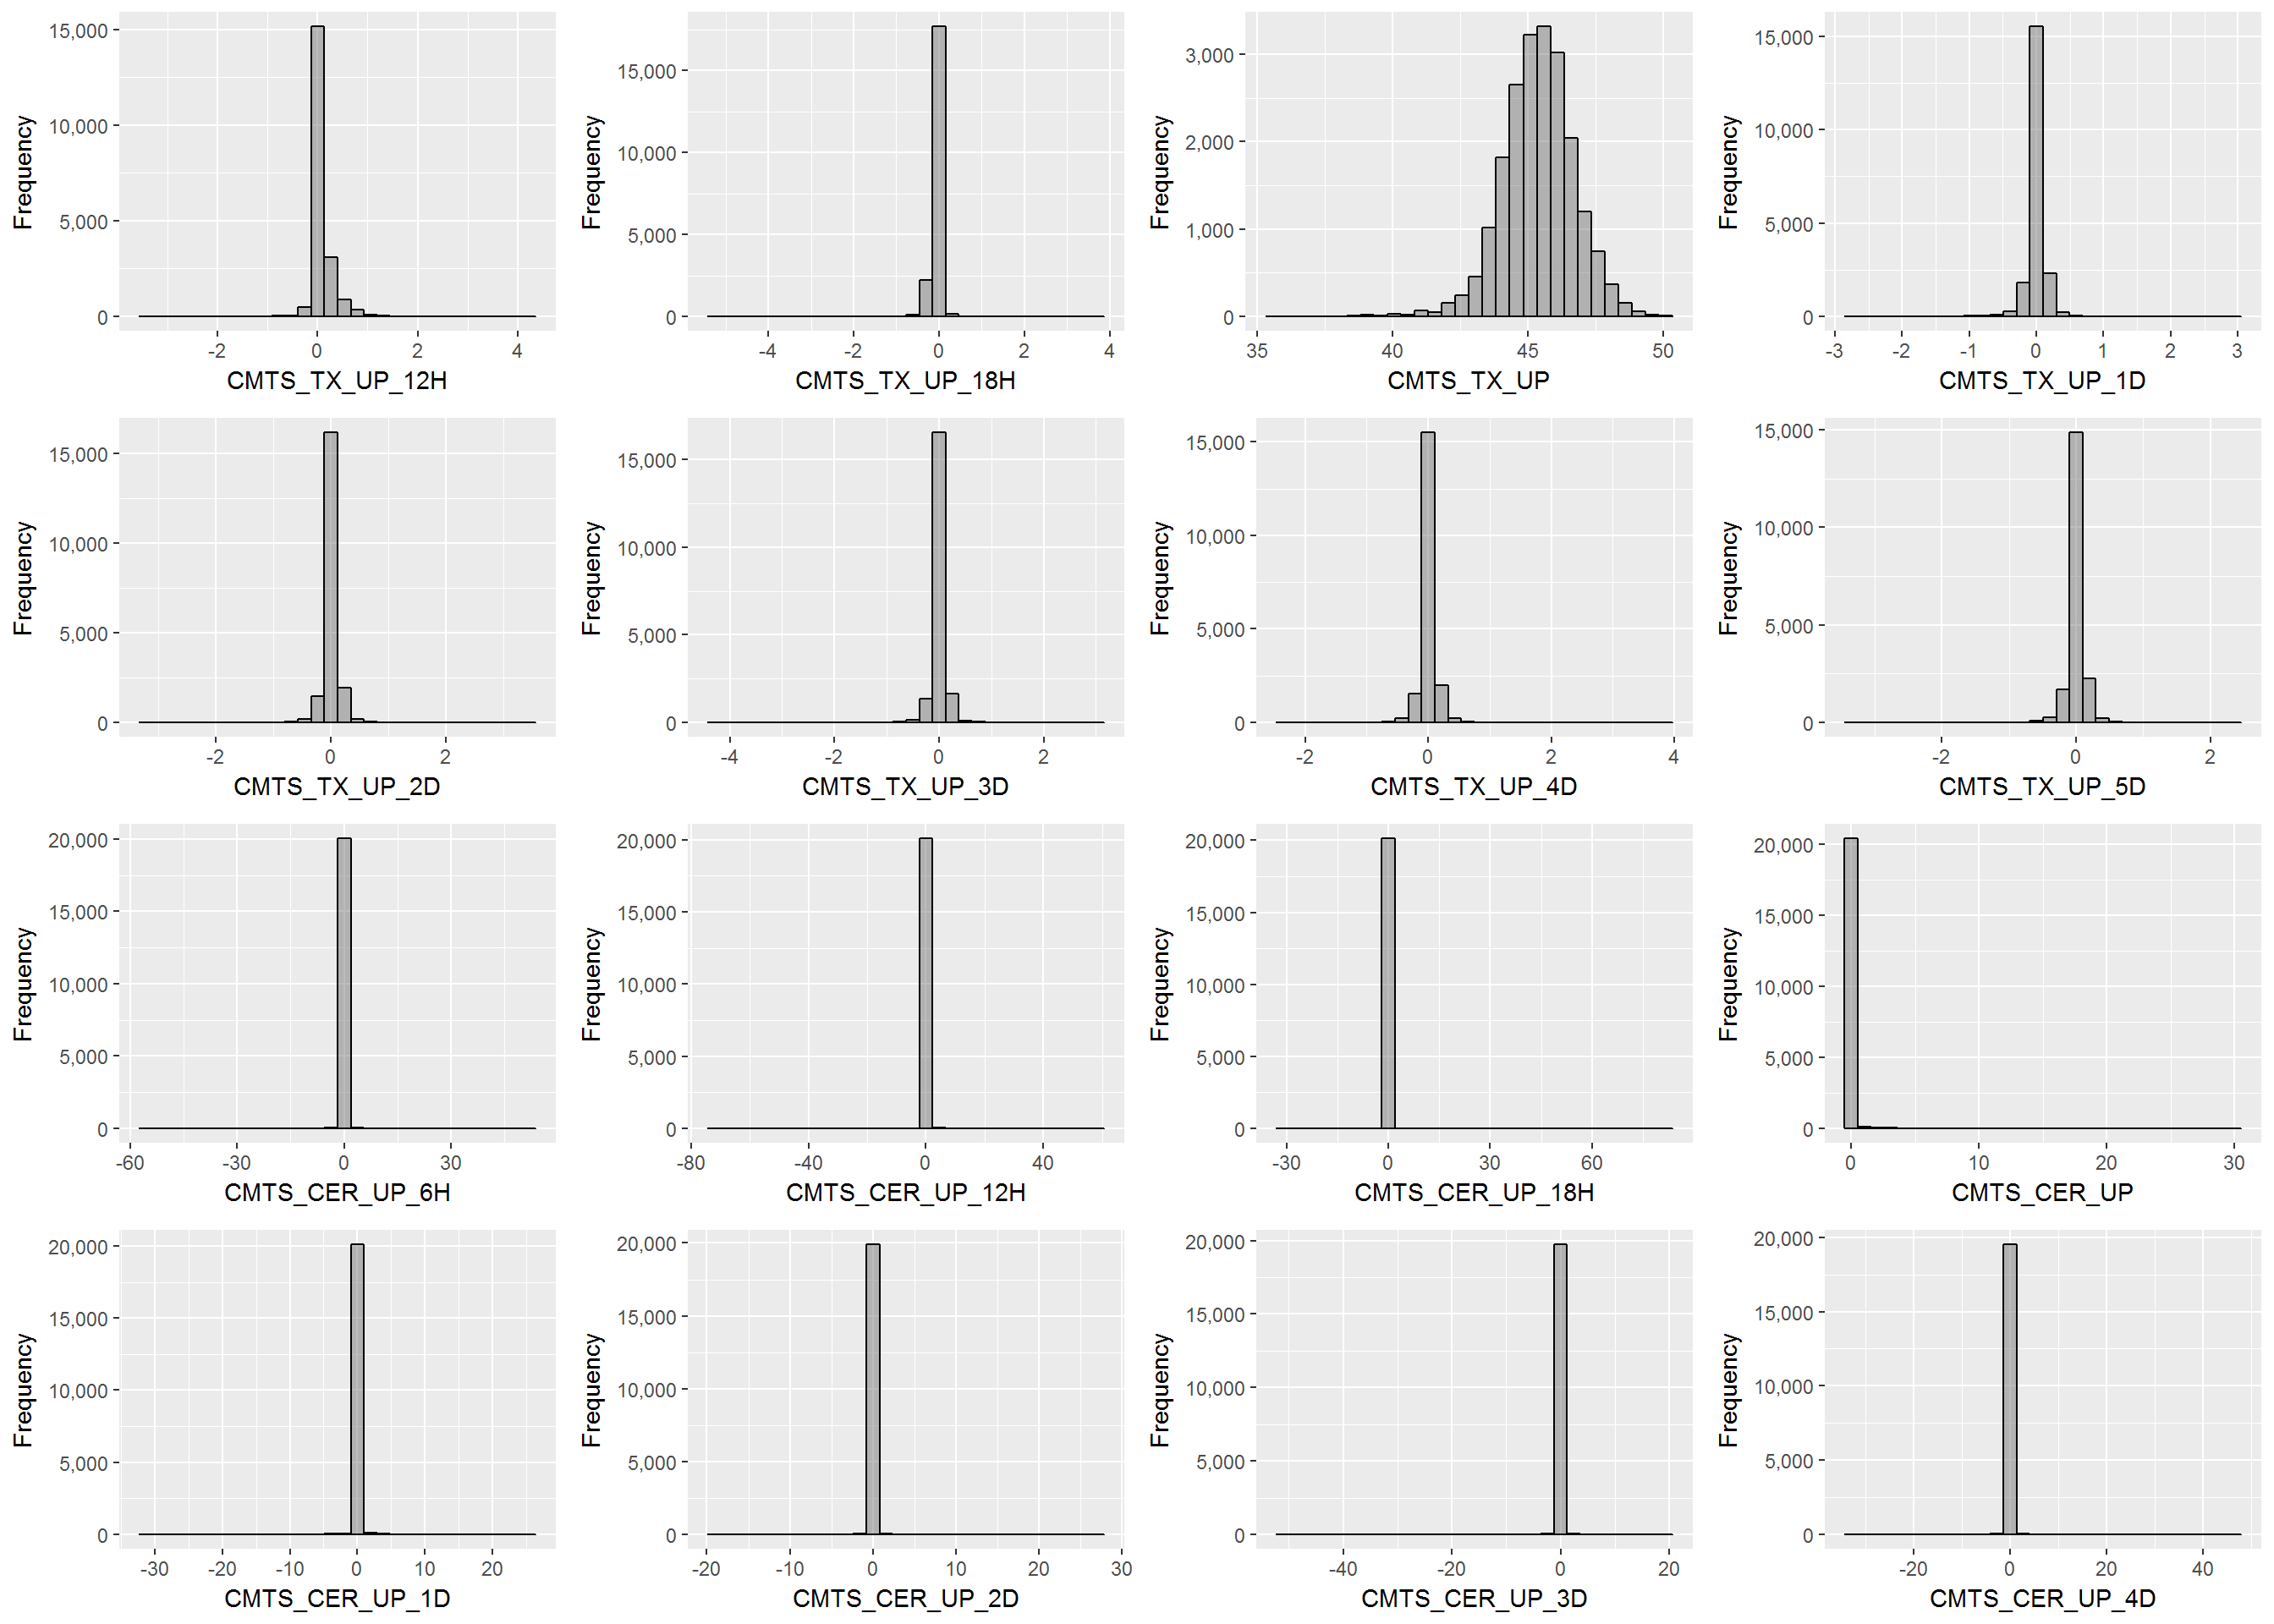
\includegraphics[width=1\linewidth]{continuous-13}
    \end{center}
    \caption{Part 13}
    \label{continuous-13}
\end{figure}

\begin{figure}[ht]
    \begin{center}
    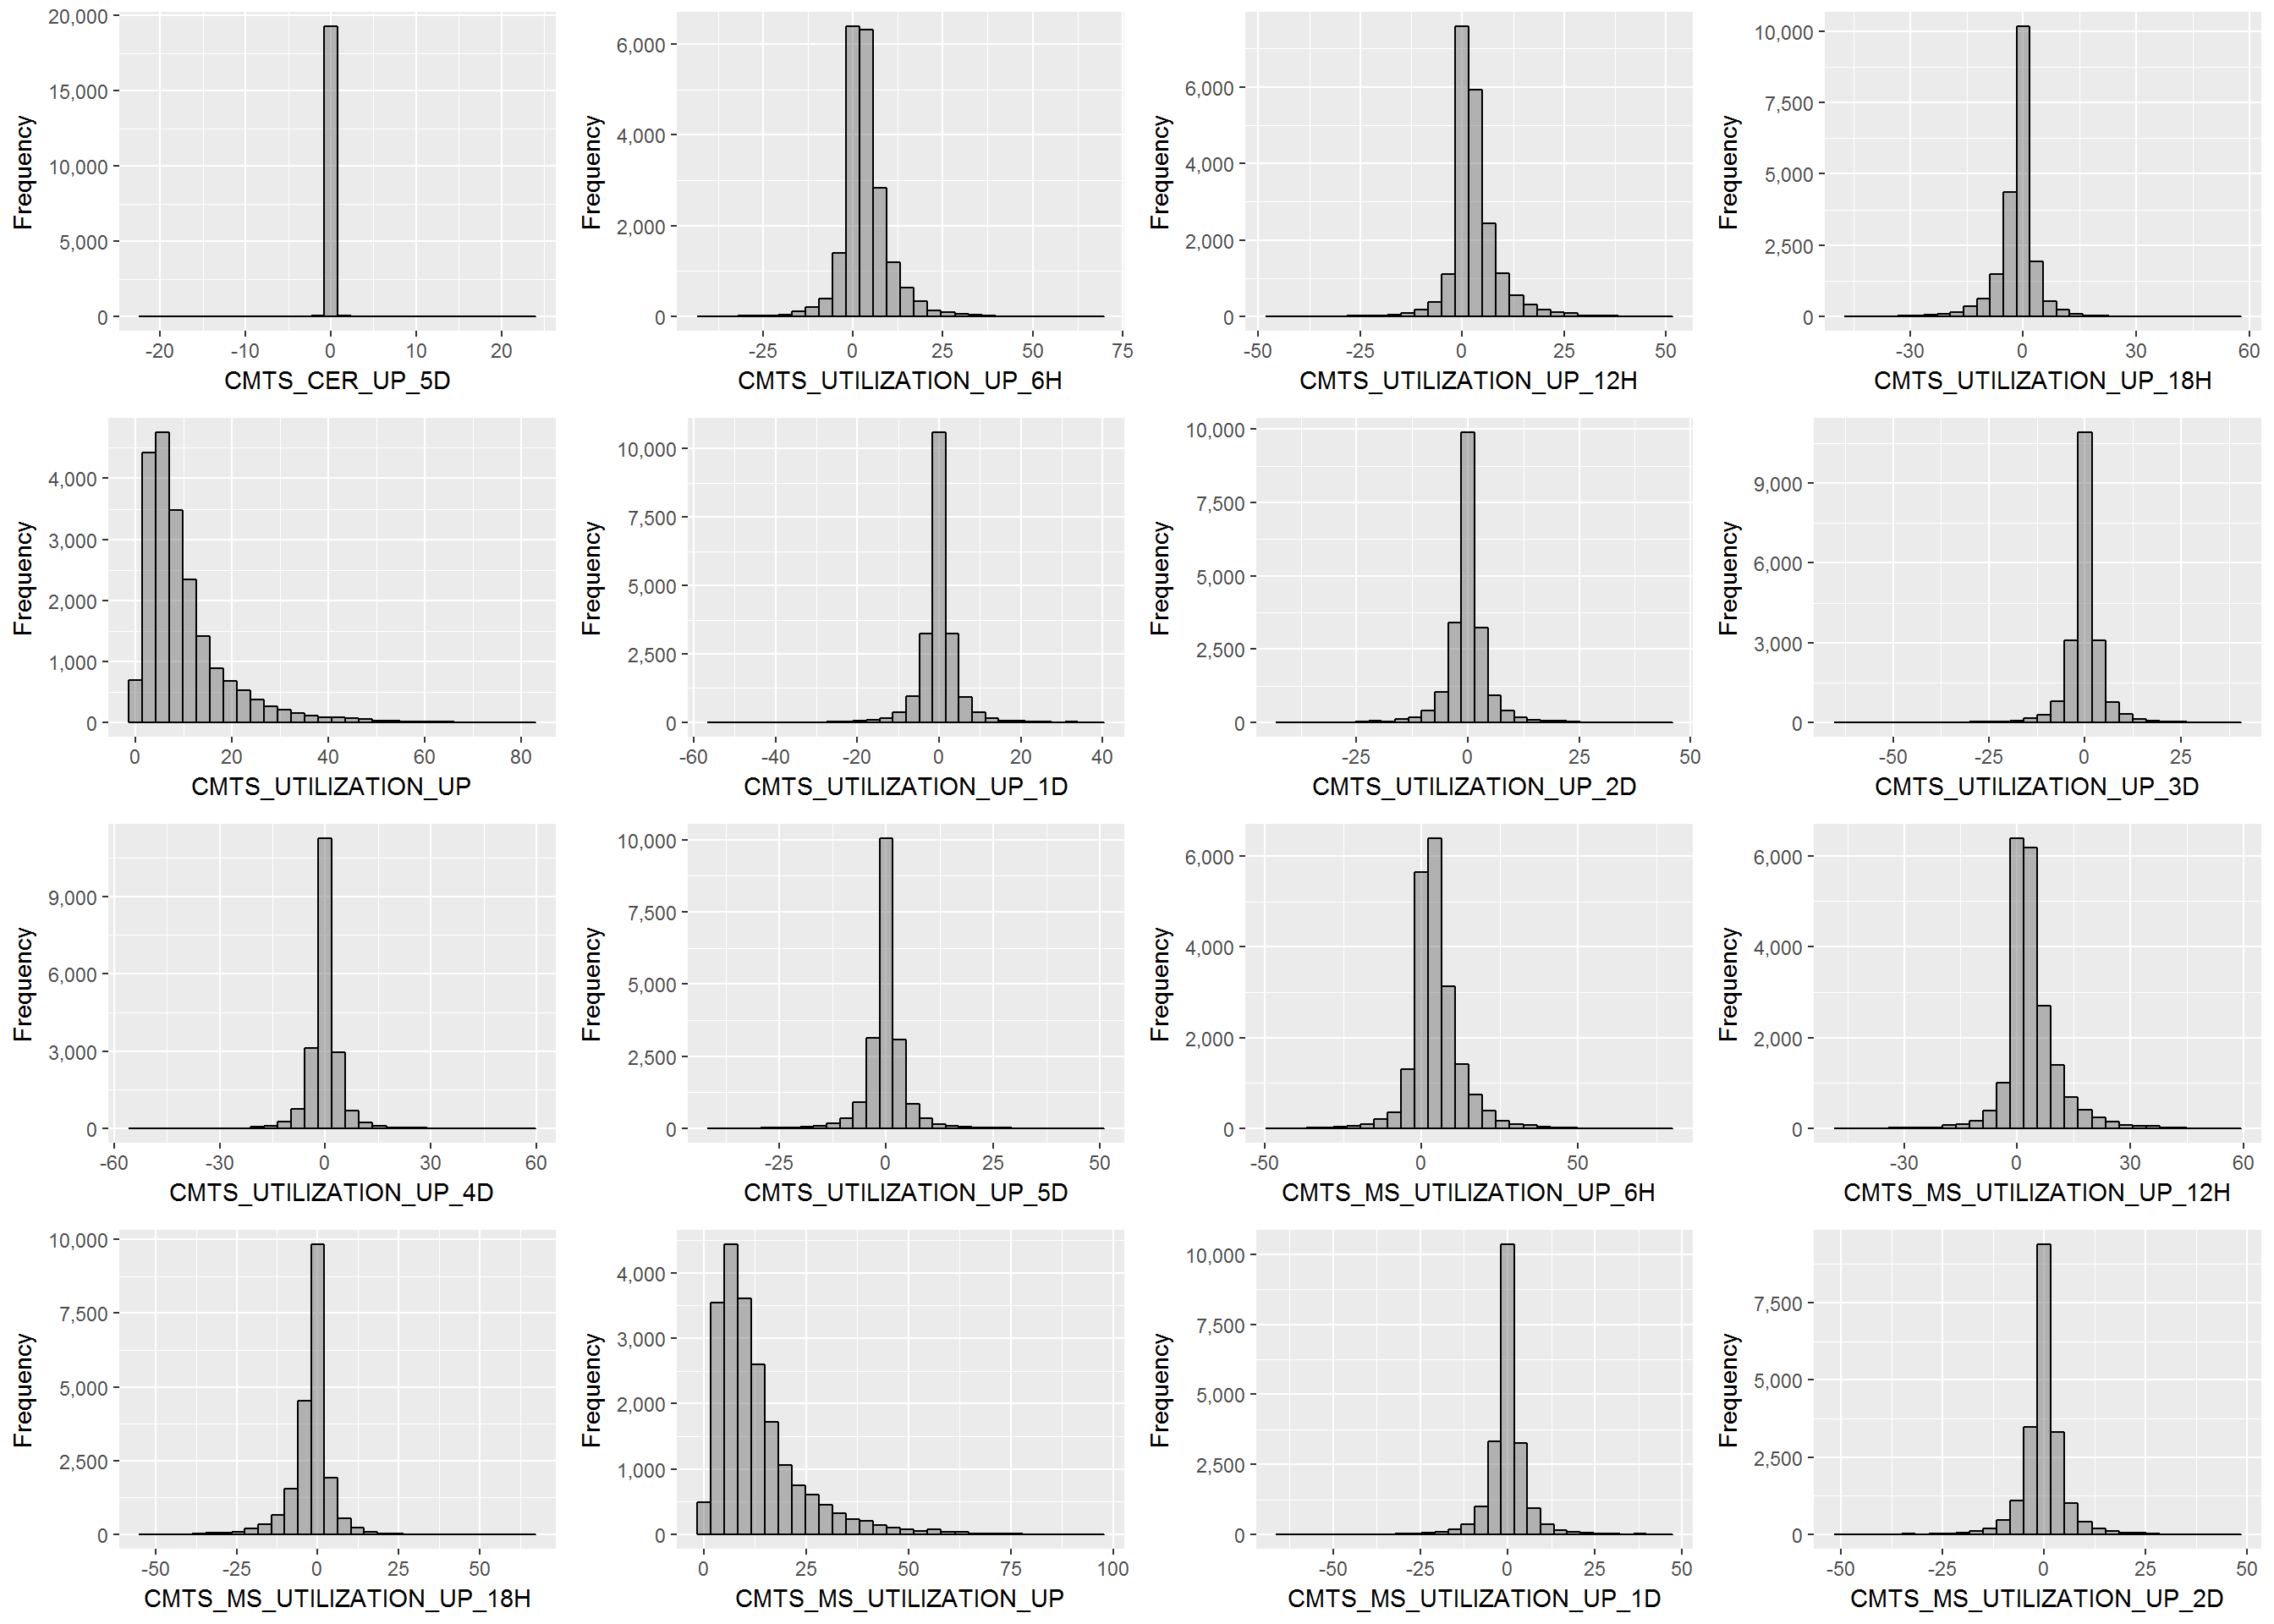
\includegraphics[width=1\linewidth]{continuous-14}
    \end{center}
    \caption{Part 14}
    \label{continuous-14}
\end{figure}

\begin{figure}[ht]
    \begin{center}
    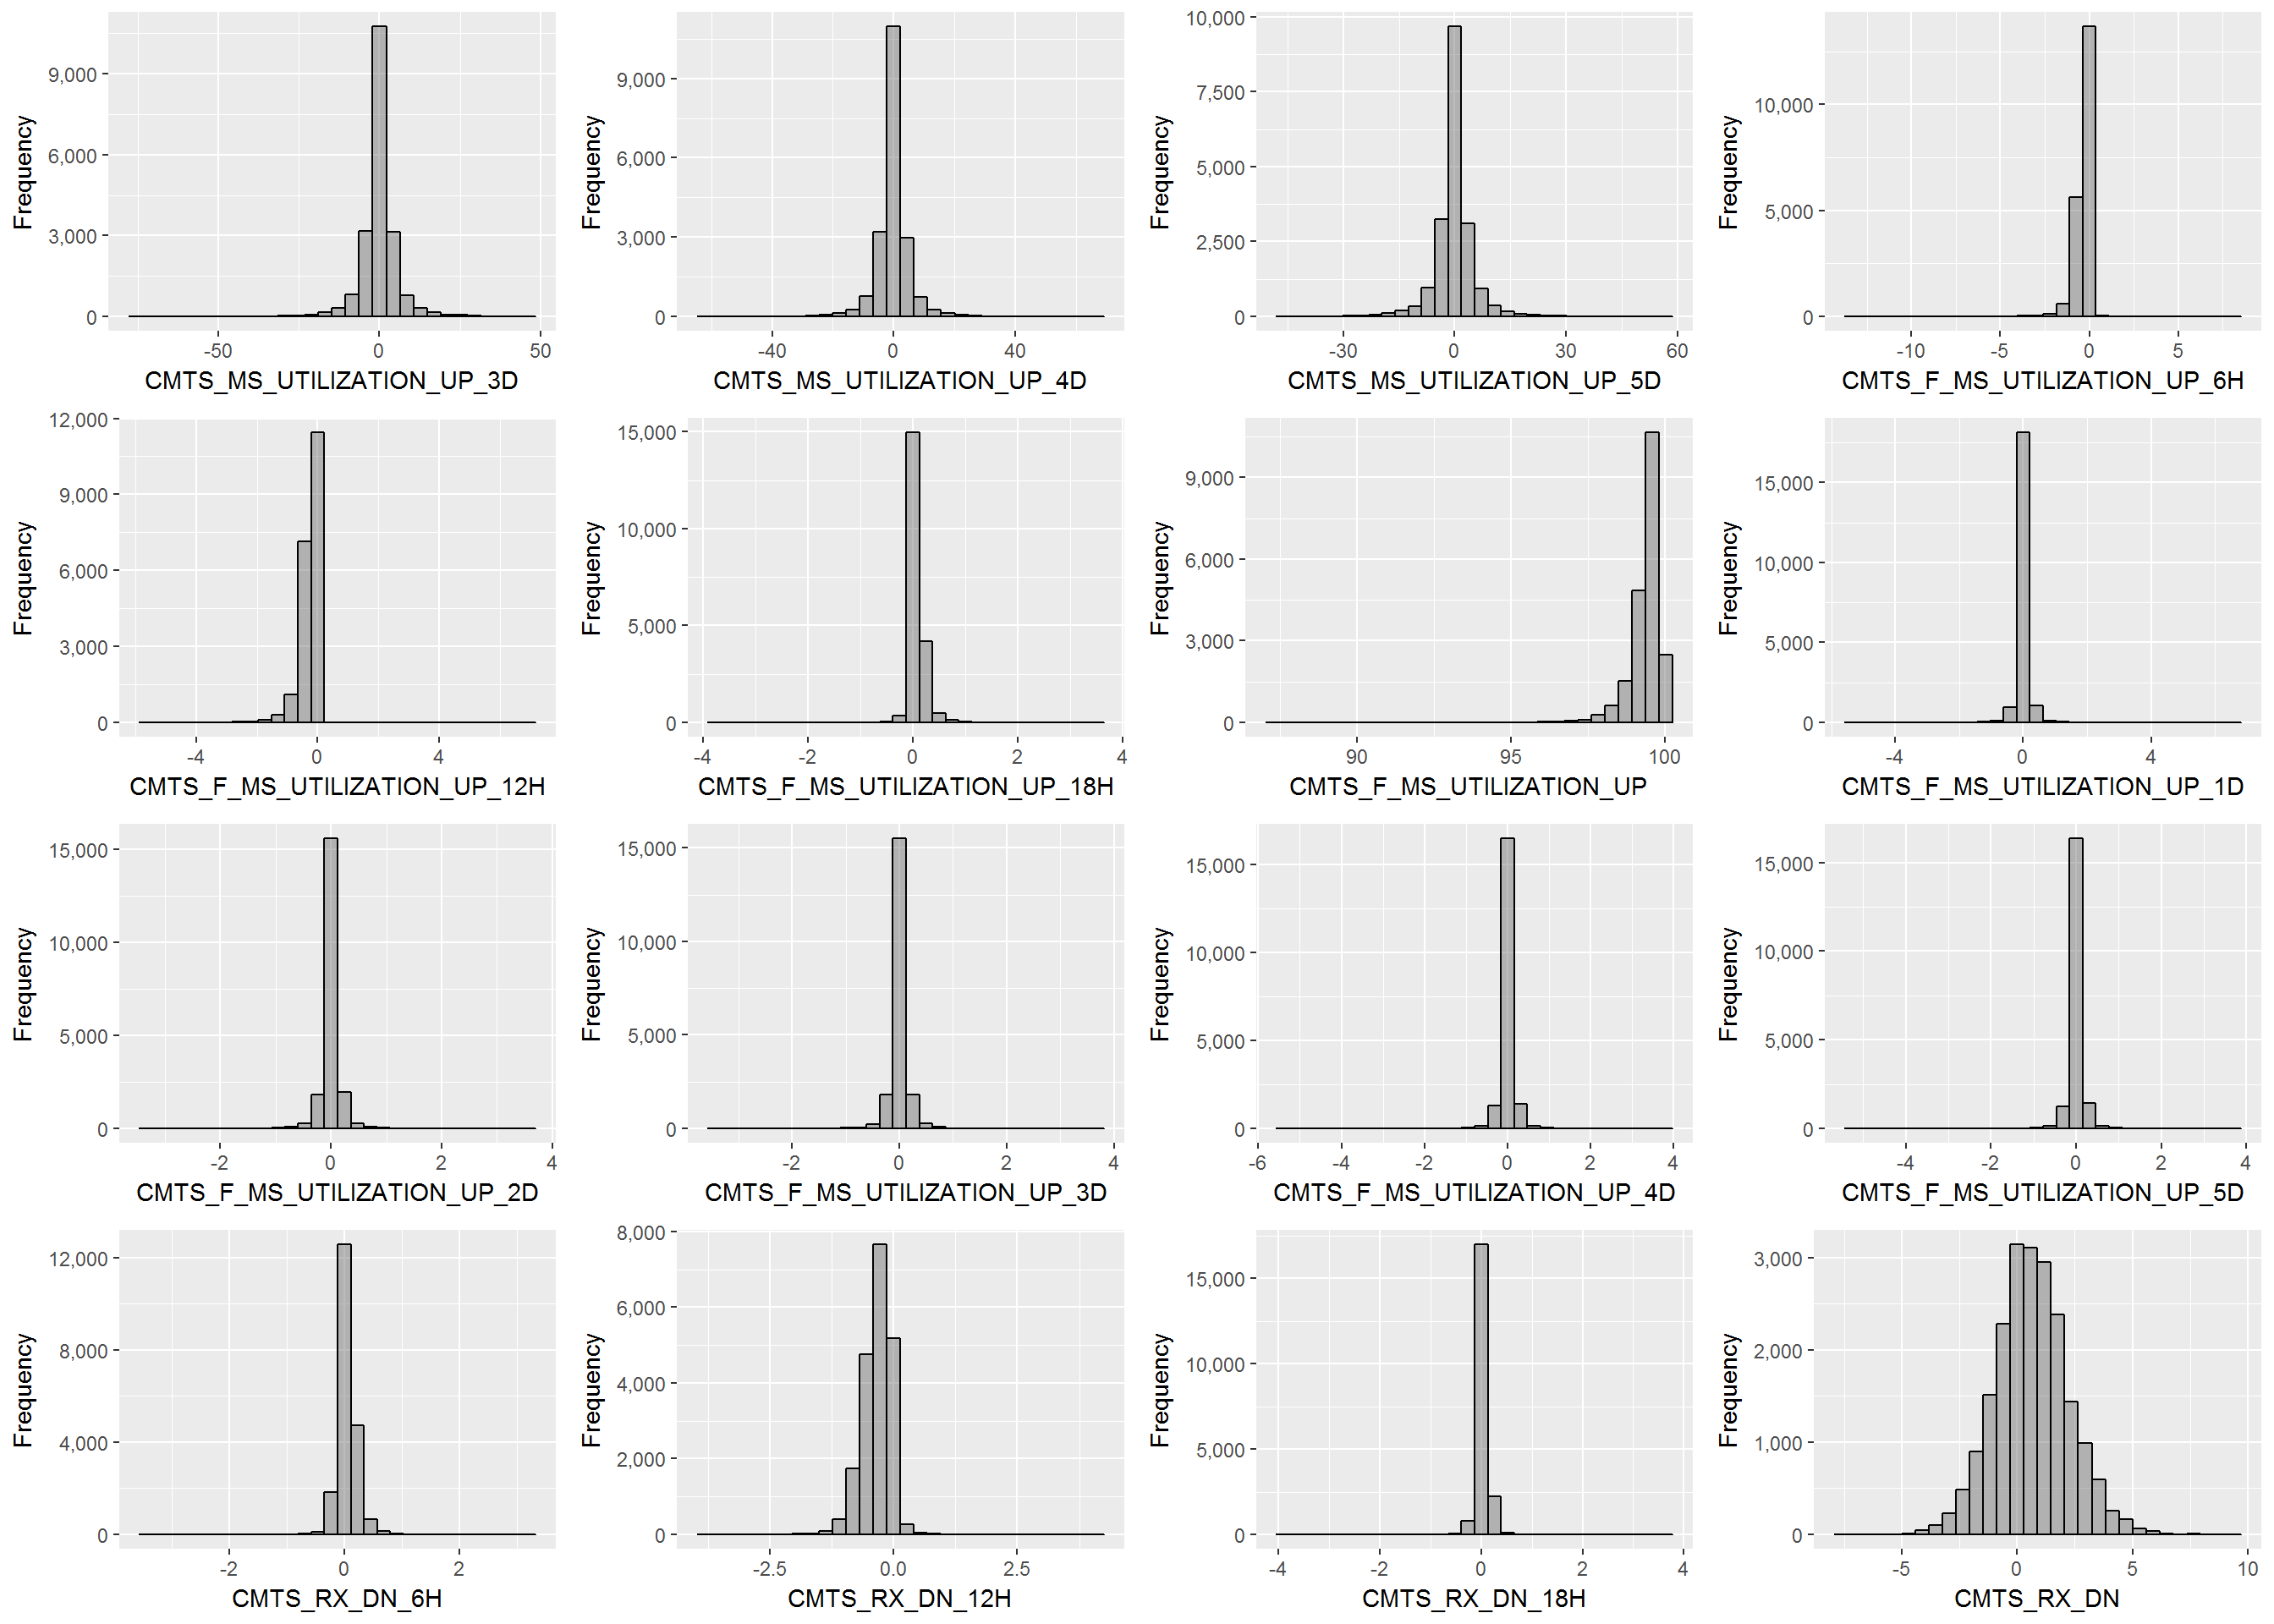
\includegraphics[width=1\linewidth]{continuous-15}
    \end{center}
    \caption{Part 15}
    \label{continuous-15}
\end{figure}

\begin{figure}[ht]
    \begin{center}
    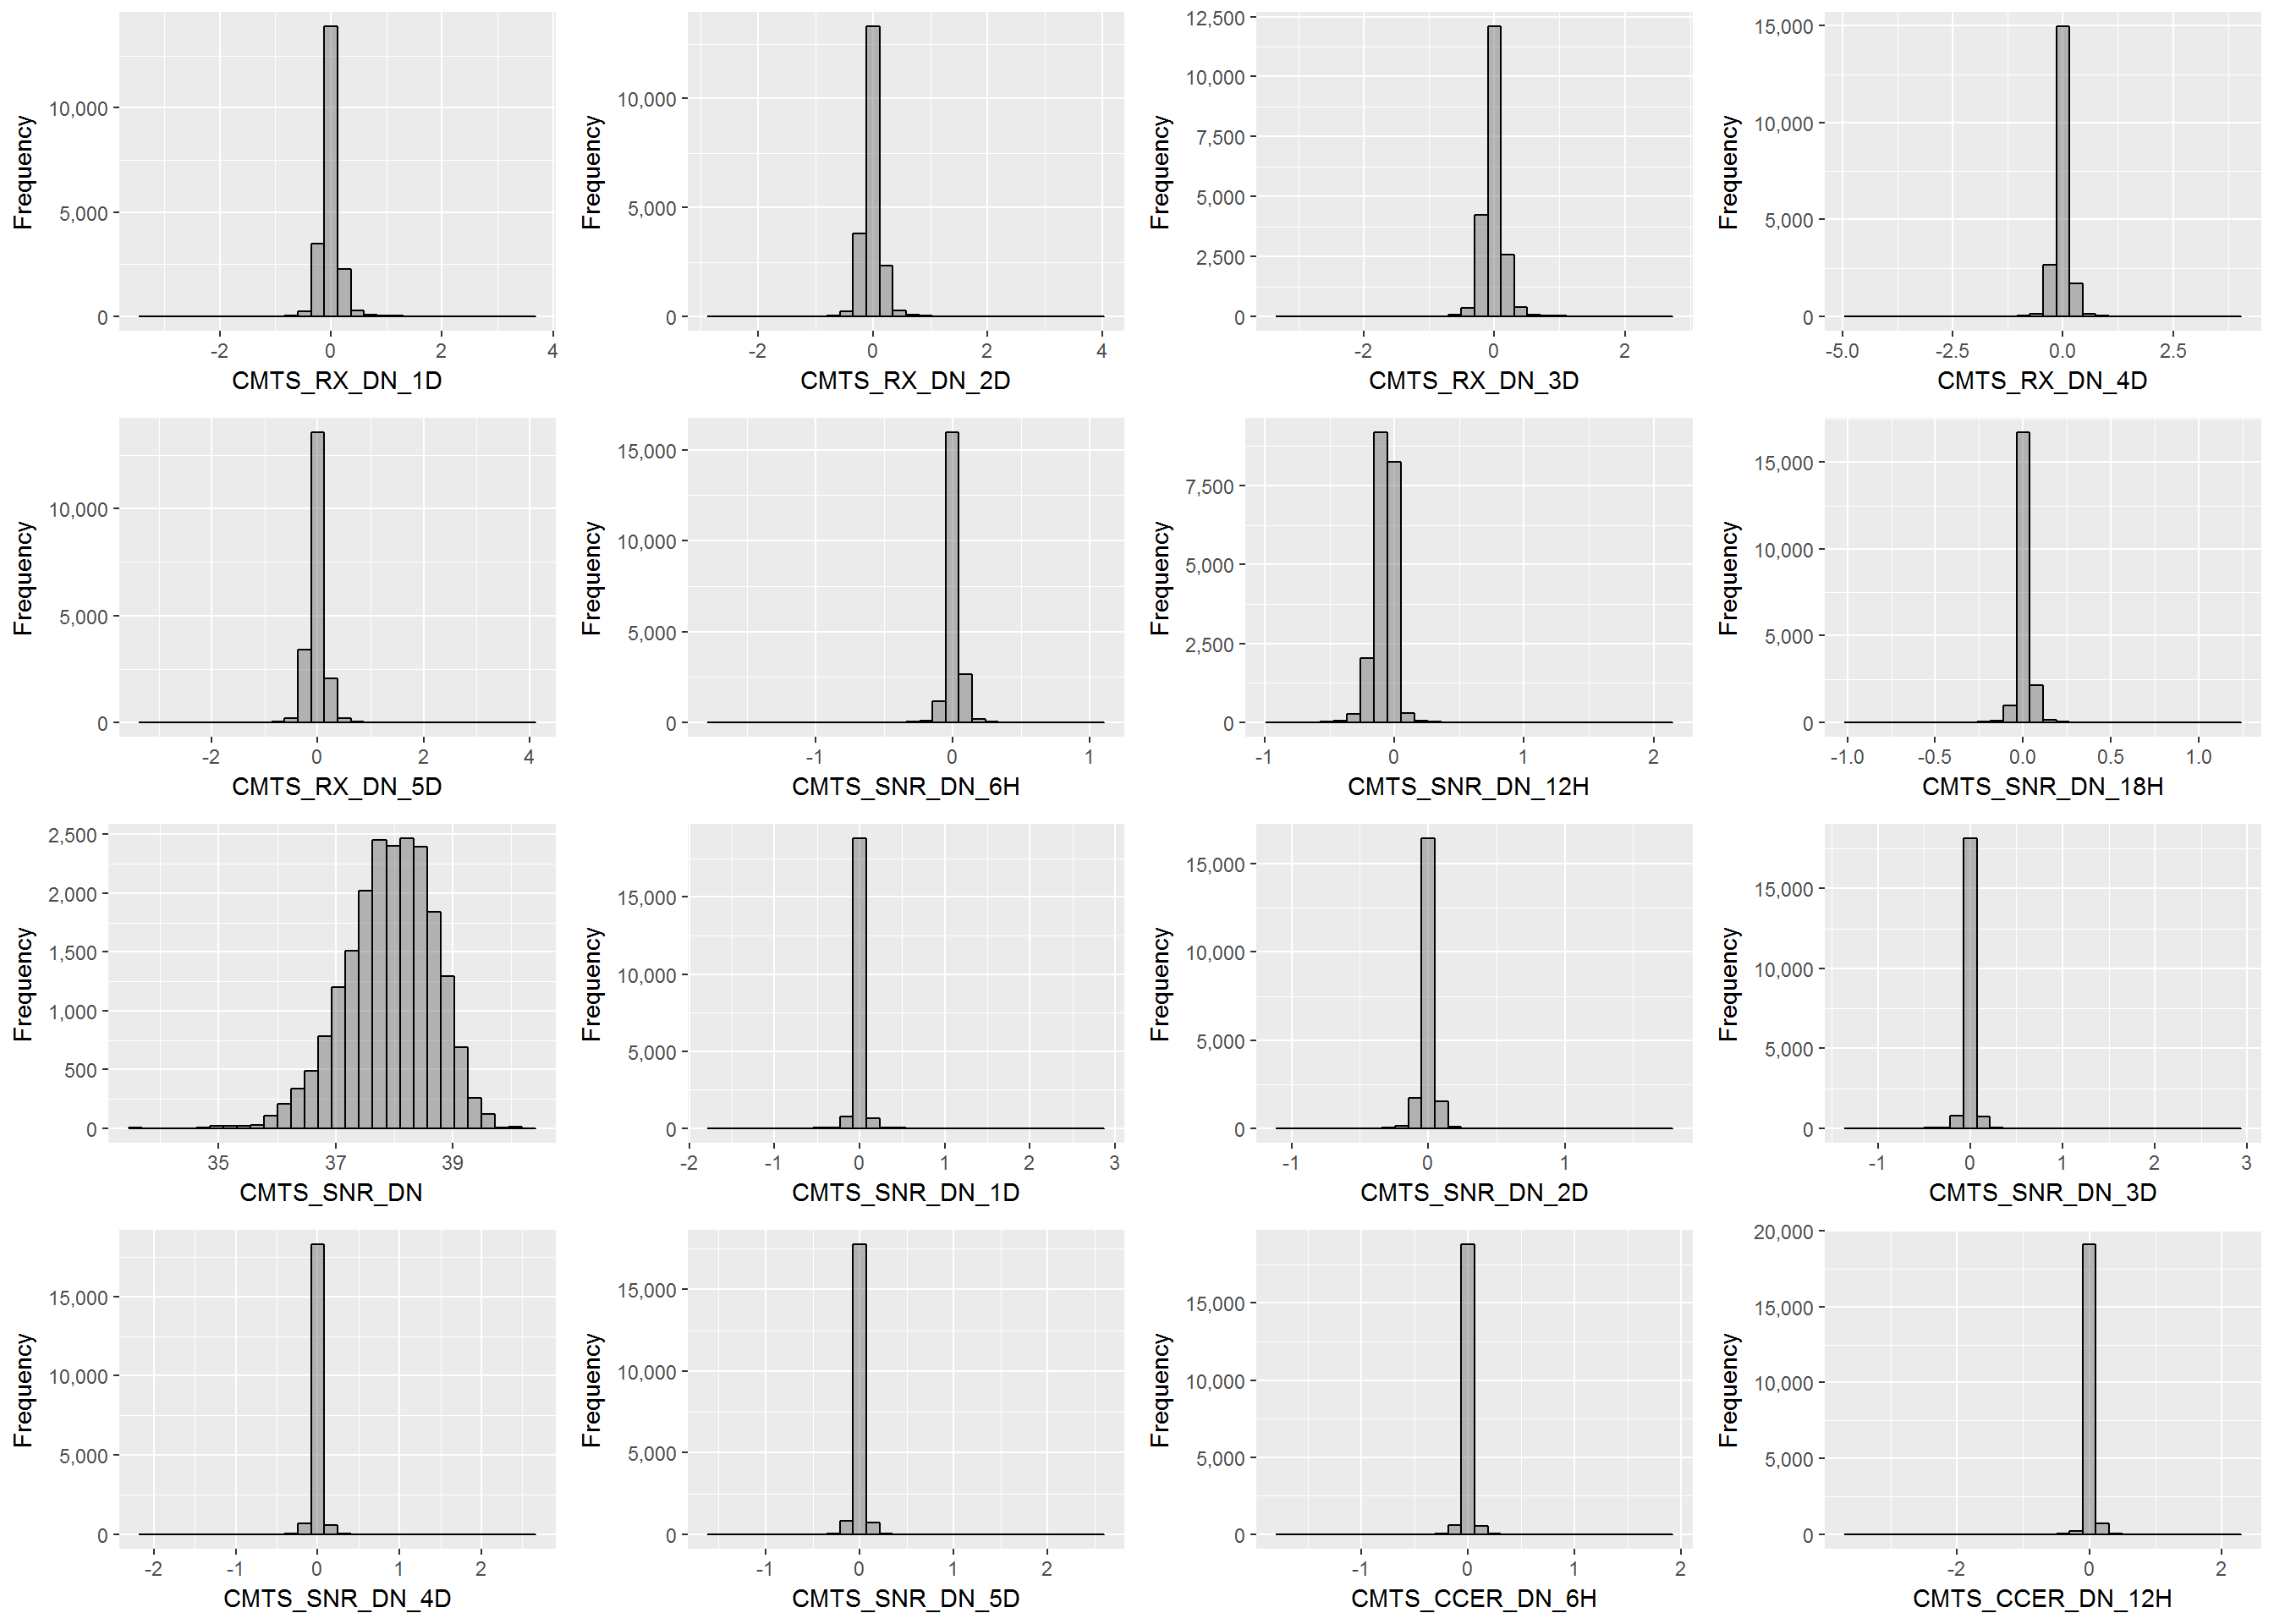
\includegraphics[width=1\linewidth]{continuous-16}
    \end{center}
    \caption{Part 16}
    \label{continuous-16}
\end{figure}

\begin{figure}[ht]
    \begin{center}
    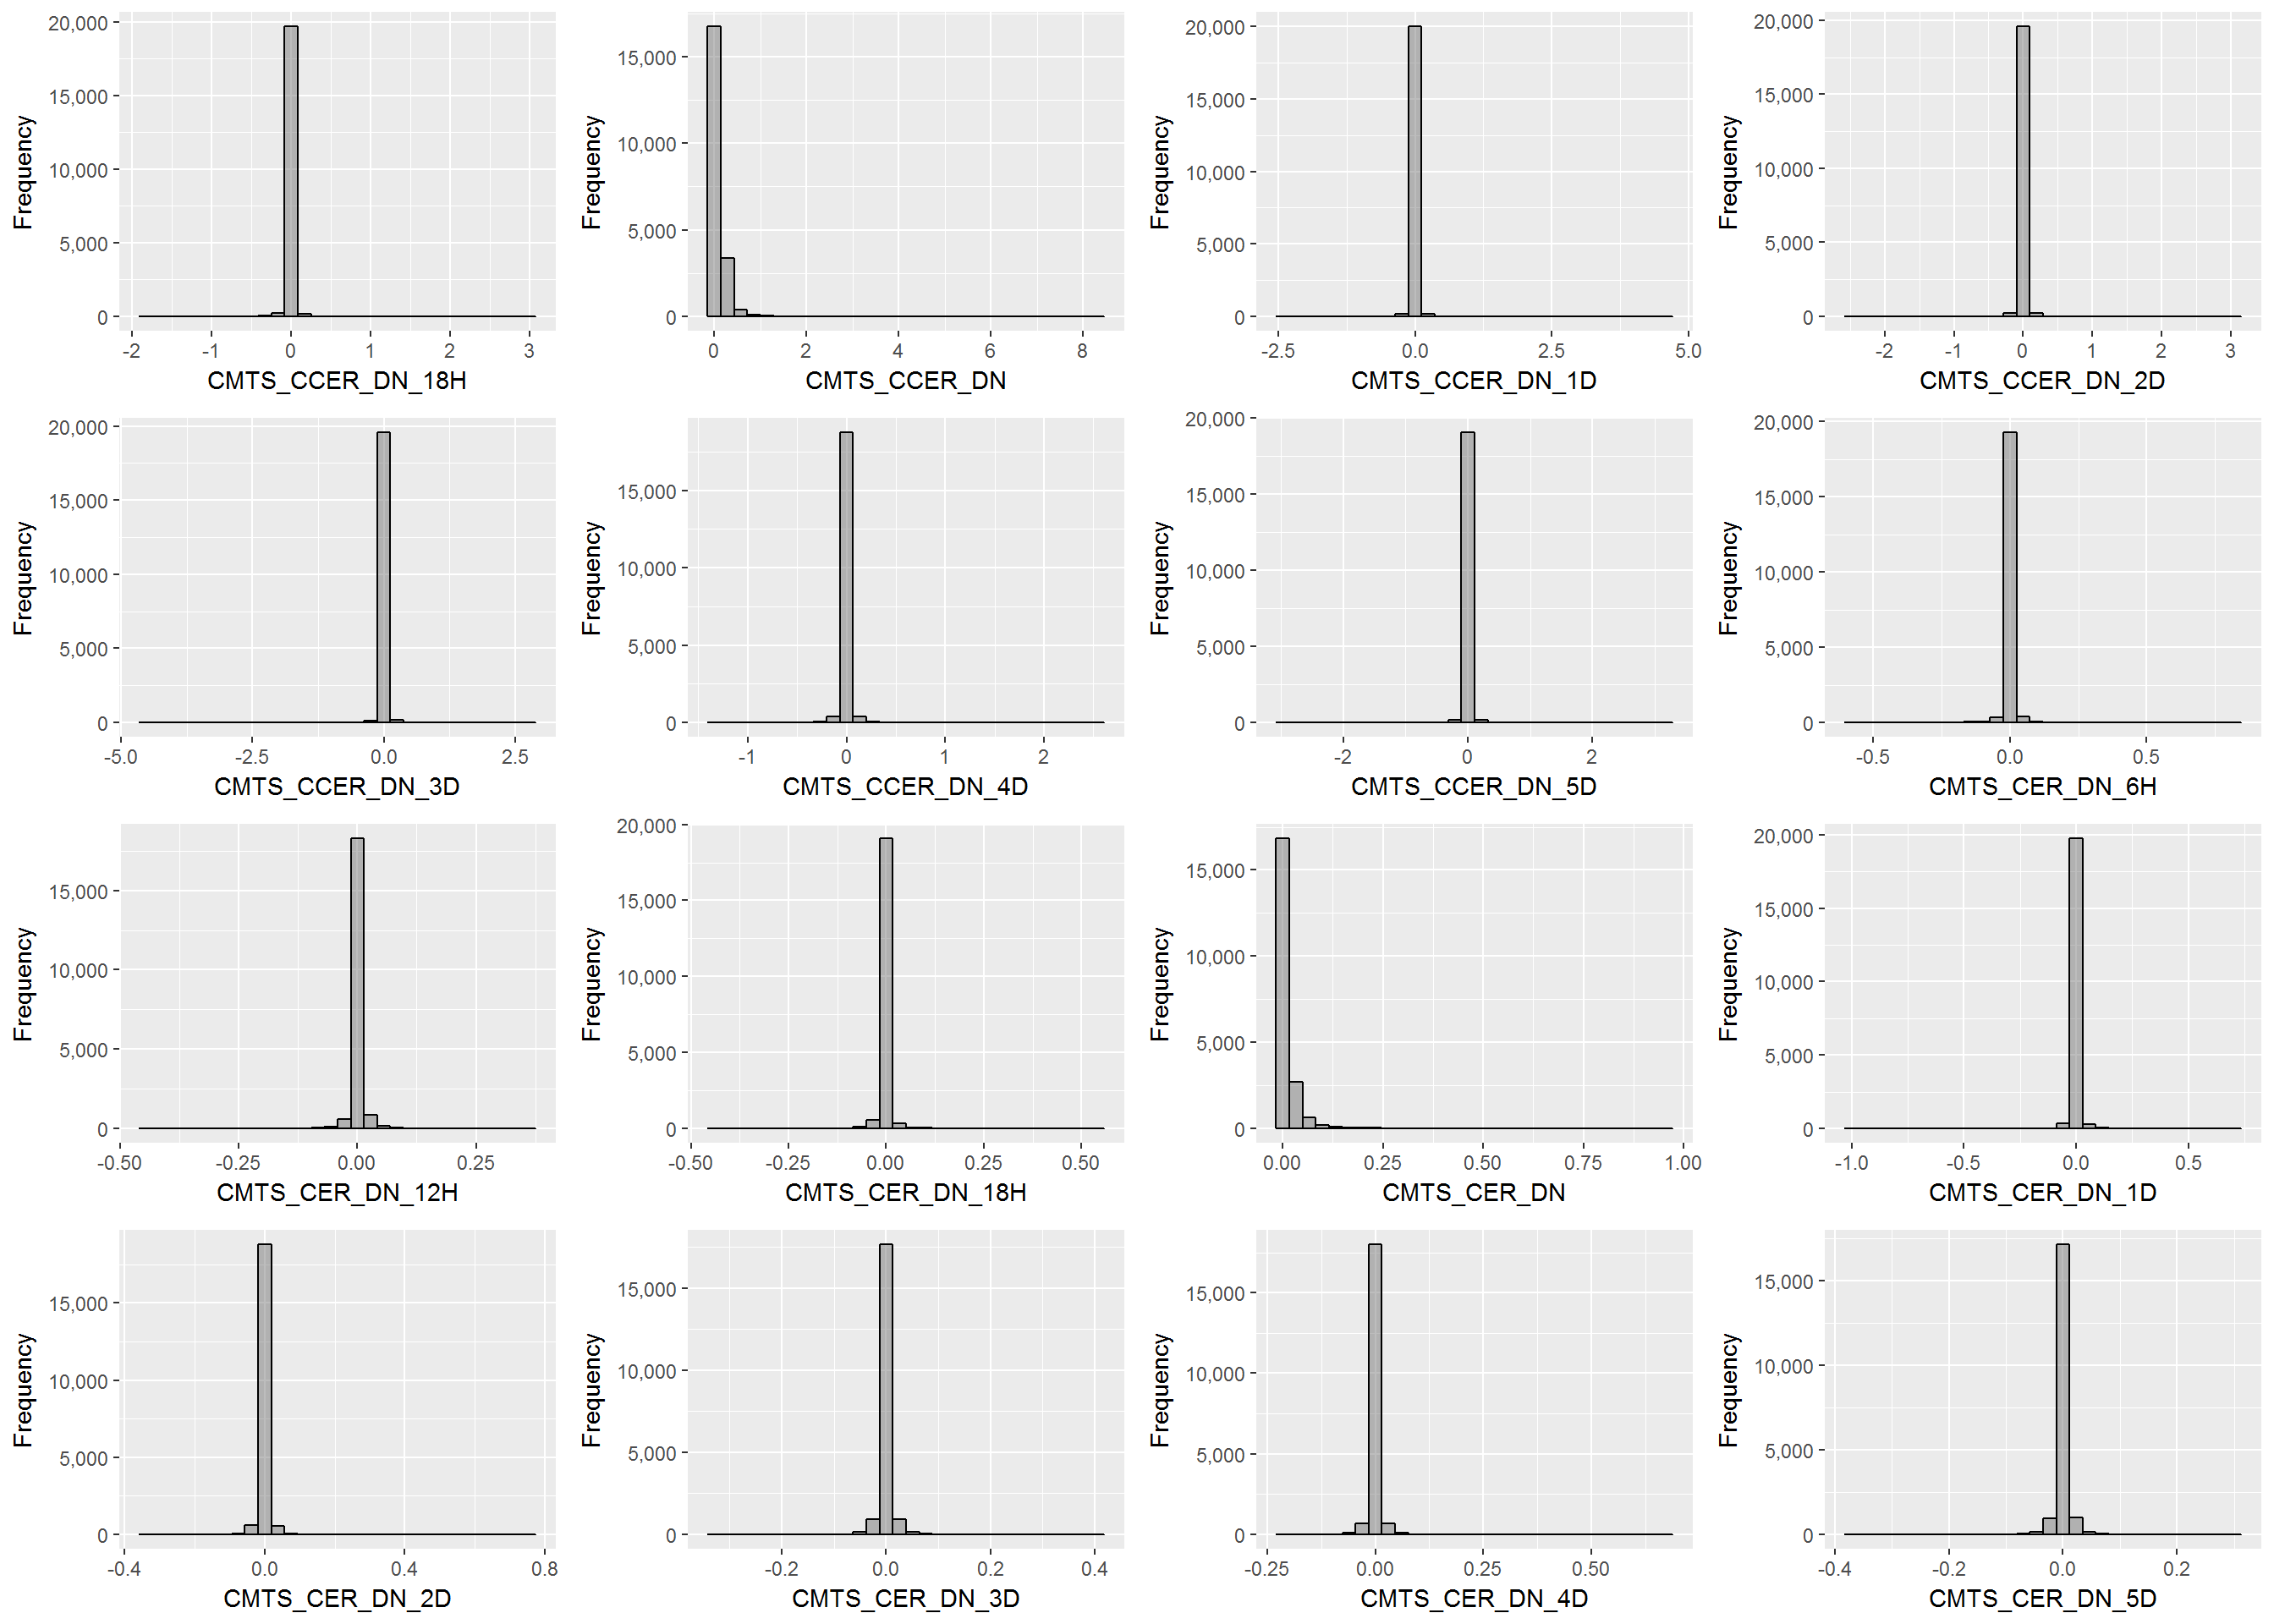
\includegraphics[width=1\linewidth]{continuous-17}
    \end{center}
    \caption{Part 17}
    \label{continuous-17}
\end{figure}

\begin{figure}[ht]
    \begin{center}
    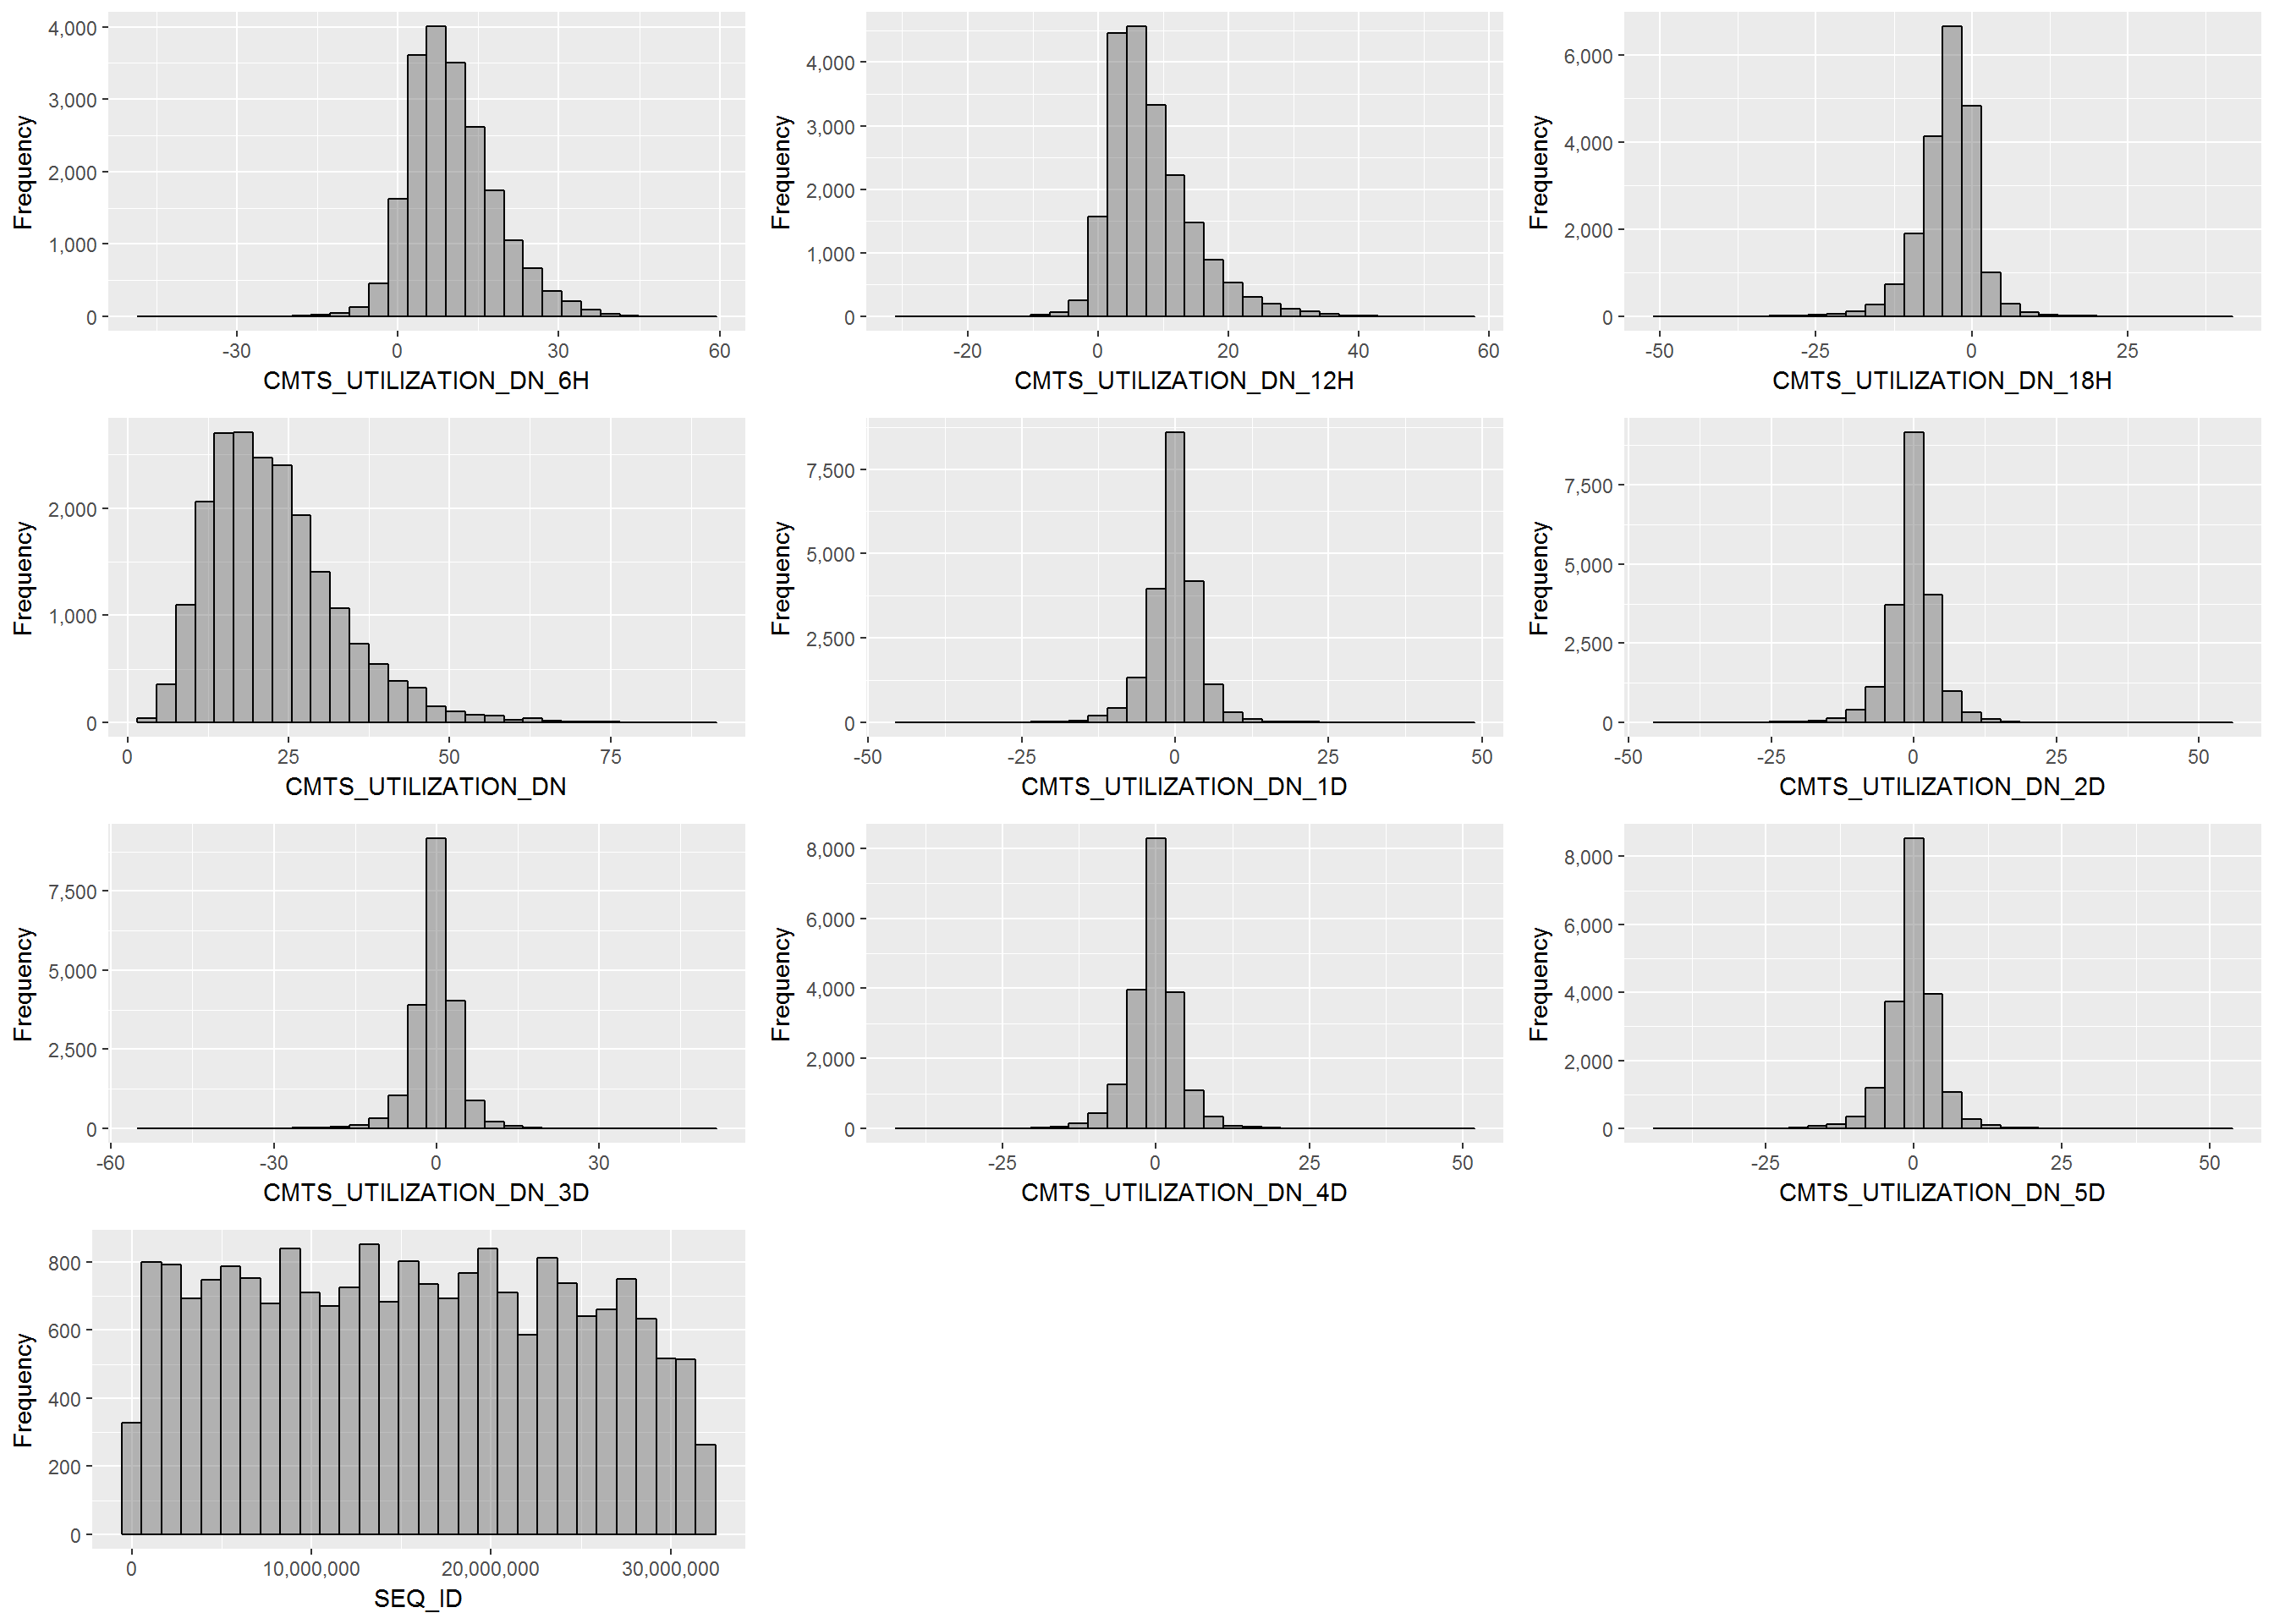
\includegraphics[width=1\linewidth]{continuous-18}
    \end{center}
    \caption{Part 18}
    \label{continuous-18}
\end{figure}

\section{Categorical Variables - Frequency Plots}
\label{sec:categorical}
Figure~\ref{categorical} displays the distribution of categorical variables.
\begin{figure}[ht]
    \begin{center}
    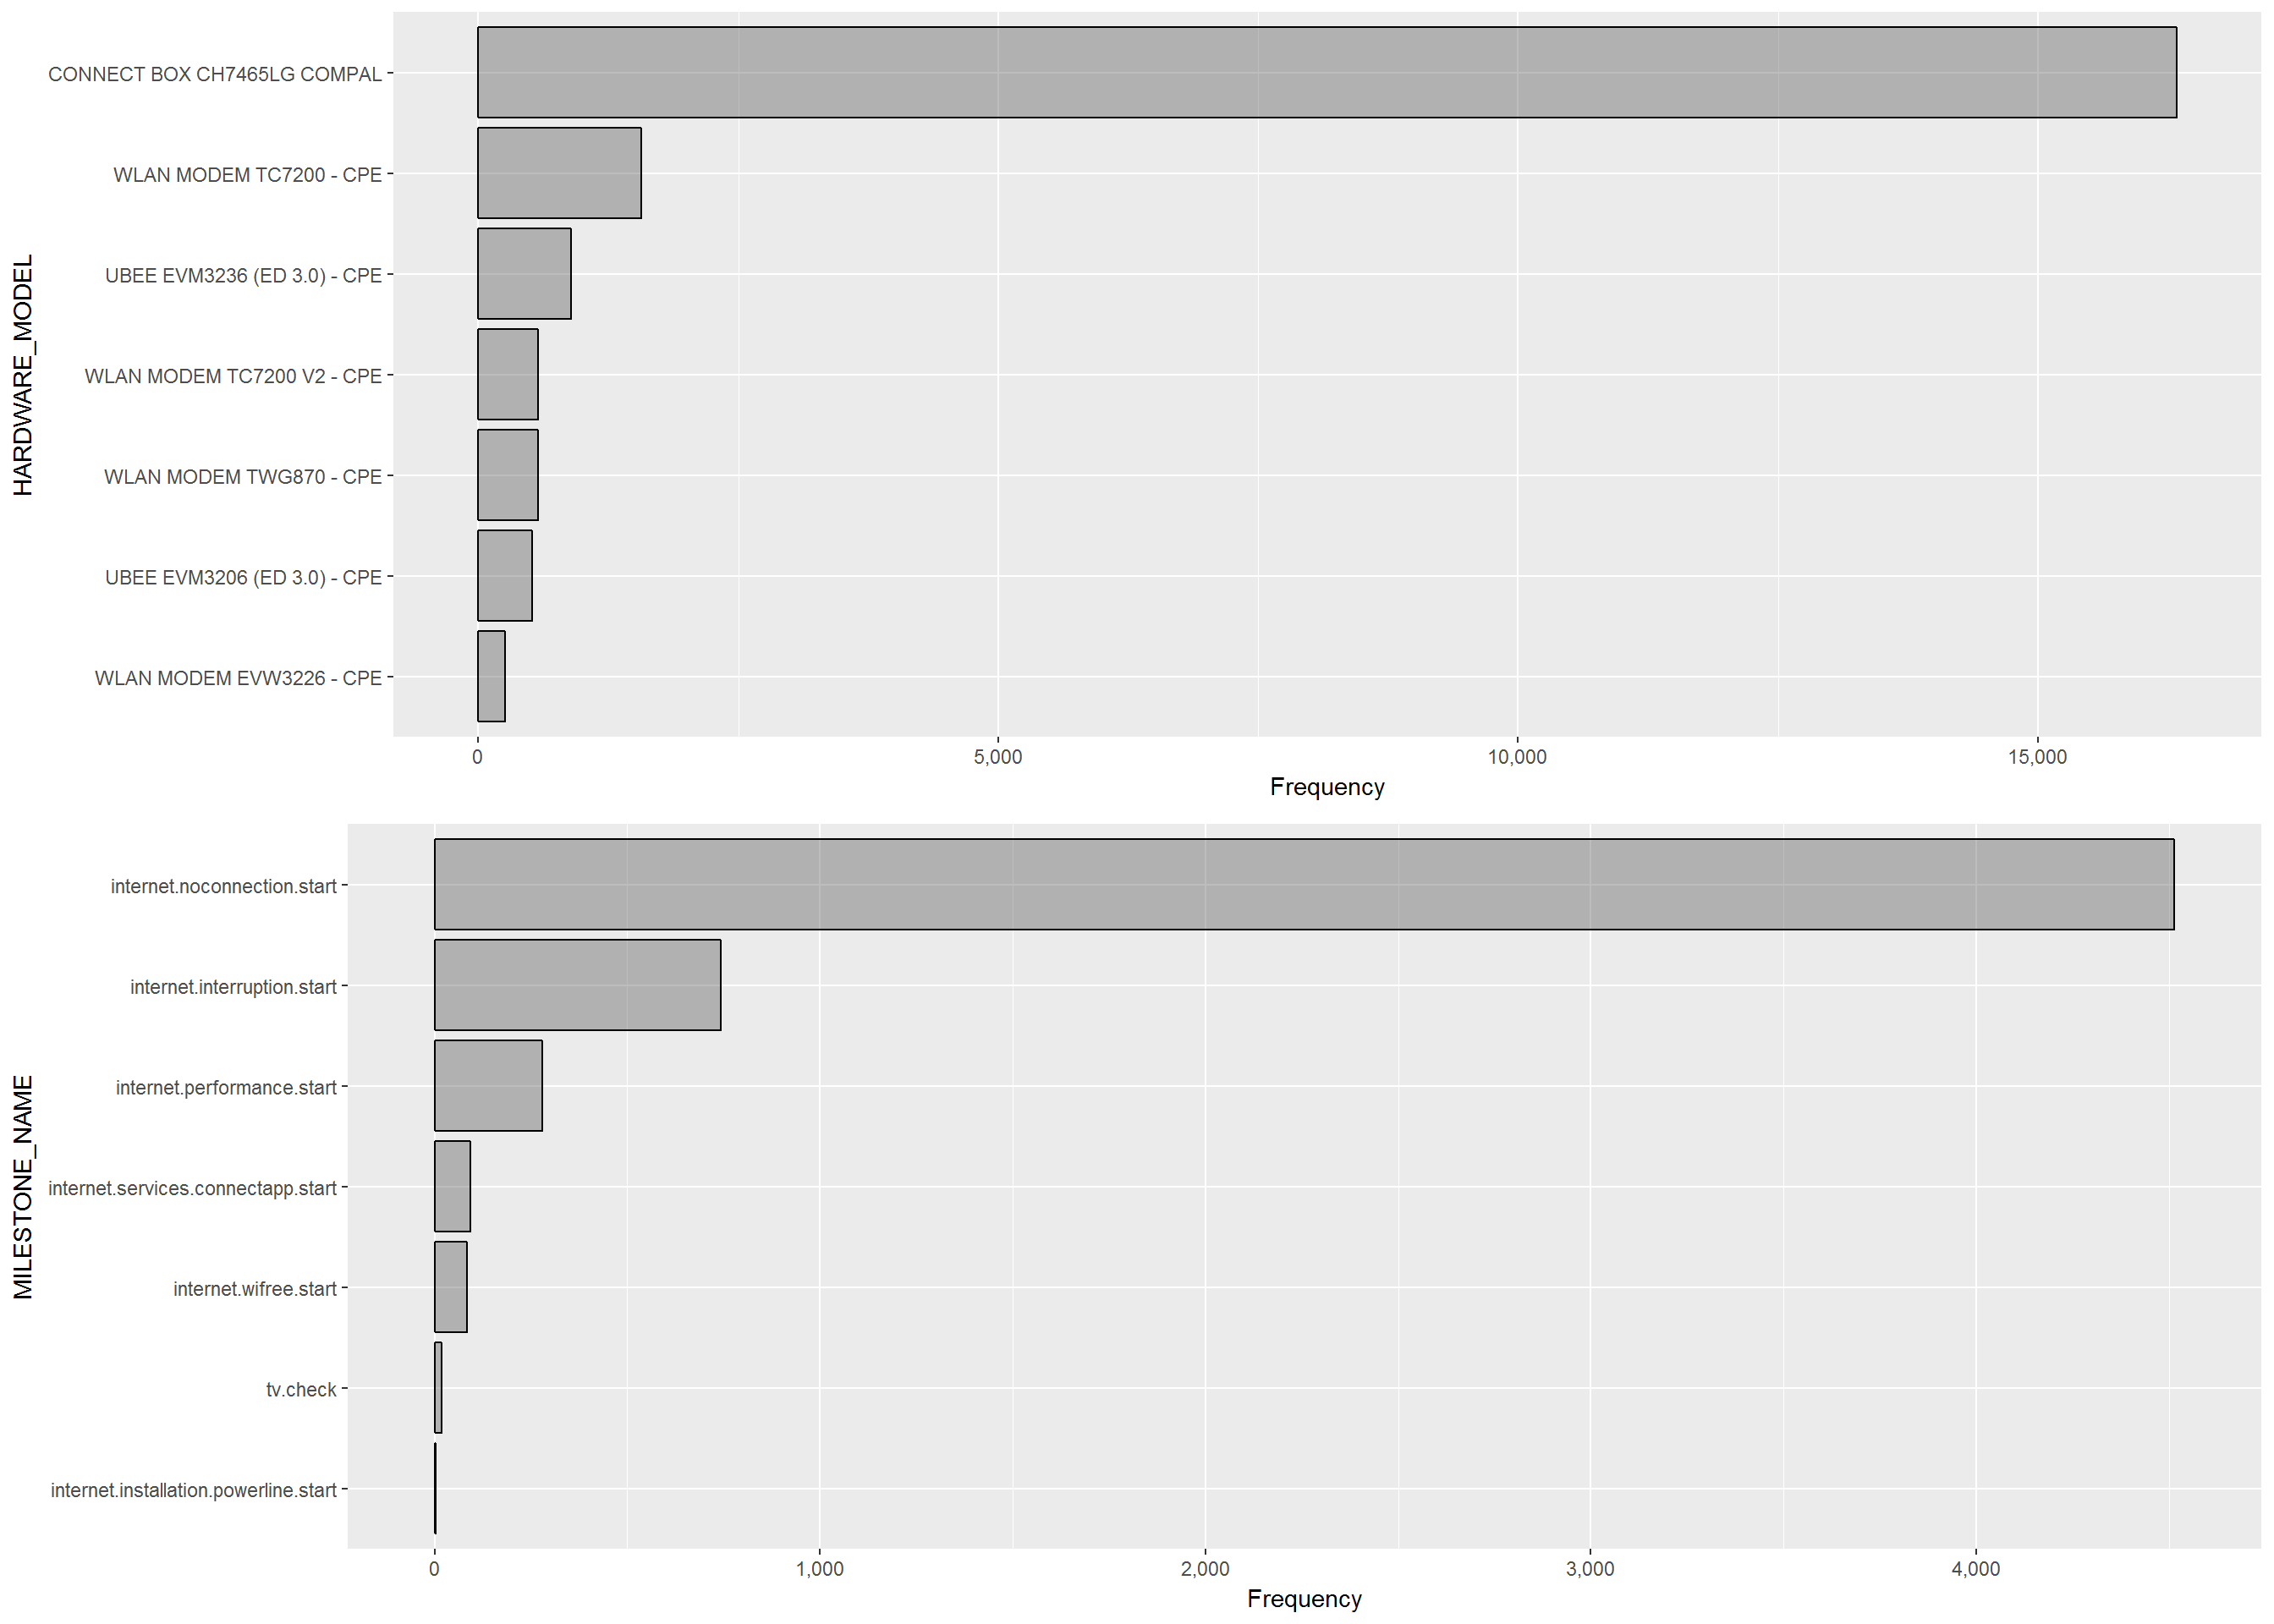
\includegraphics[width=1\linewidth]{categorical-1}
    \end{center}
    \caption{Categorical variables}
    \label{categorical}
\end{figure}


